% -*- root: main.tex -*-
%-------------------------------------------------------------------------------
\chapterimage{chapter_head_10.pdf} 

%-------------------------------------------------------------------------------
\chapter{모바일 로봇}

%-------------------------------------------------------------------------------
\section{ROS 로봇}\index{ROS 로봇}

%-------------------------------------------------------------------------------
\subsection{ROS 지원 로봇}\index{ROS 지원 로봇}

ROS 에서 지원하는 로봇은 관련 위키 http://wiki.ros.org/Robots 에서 찾아 볼 수 있다. 그 수는 2014년 6월 현재 120여 가지에 달한다. 이 중 일부는 일반 유저가 공개한 커스텀 로봇이 포함되어 있기는 하지만 하나의 시스템이 지원하는 로봇이라는 점을 생각하면 적지 않은 수이다. 그 중 가장 많이 알려져 있는 로봇으로는 윌로우게러지(willowgarage)\footnote{http://www.willowgarage.com/}가 개발한 PR2와 터틀봇이 유명하다. 이 둘 모두 윌로우게러지 또는 OSRF(Open Source Robotics Foundation)\footnote{http://www.osrfoundation.org/} 가 개발에 참여한 로봇으로 ROS의 공식 지정 로봇이라고 봐도 이상하지 않다. 이 중에서 우리는 ROS의 학습에 있어서 실습을 터틀봇(Turtlebot)에 사용되는 거북이(Kobuki)를 중심으로 실습을 해볼 수 있도록 하겠다.

\begin{figure}[h]
\centering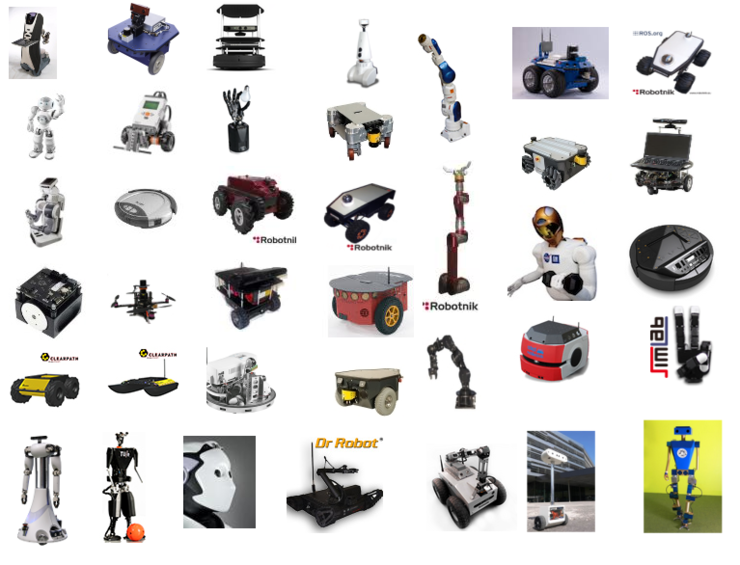
\includegraphics[width=\columnwidth]{pictures/chapter10/robots.png}
\caption{ROS Robots}
\end{figure}

%-------------------------------------------------------------------------------
\subsection{TurtleBot}\index{TurtleBot}

TurtleBot? 아마 처음 듣는 사람들도 있을 것이다. 터틀봇은 거북이 로봇 이라는 의미(?)로 우리가 사용하고 있는 ROS 의 대표적인 로봇이다. 터틀이라는 이름도 ROS의 심볼인 거북이에서 비롯된 것이다. 

\begin{figure}[h]
\centering
\includegraphics[width=0.5\columnwidth]{pictures/chapter10/turtle_icons.png}
\caption{ROS의 각 버전의 거북이 심볼}
\end{figure}

터틀봇은 ROS를 처음다루는 사람들을 위해 나온 로봇으로, 오픈 로봇공학 플랫폼에 개발자, 학생 등이 많이 사용되고 있다. 현재까지 TurtleBot 1, 2 가 나왔으며, TurtlBot 1은 iRobot 사의 Roomba, TurtleBot 2는 Yujinrobot의 Kobuki를 하드웨어로 이용하고 있다. 그리고, 3차원 데이타 수집을 위하여 Microsoft 사의 Kinect 또는 Asus 의 Xition 을 사용하고 있다.

\begin{figure}[h]
\centering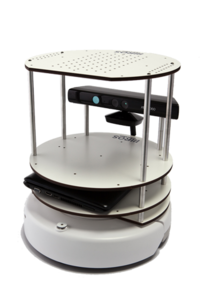
\includegraphics[height=40mm]{pictures/chapter10/turtlebot1.png}
\centering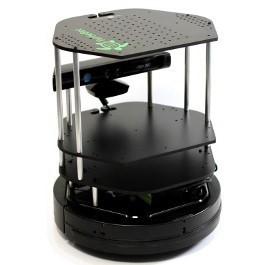
\includegraphics[height=35mm]{pictures/chapter10/turtlebot2.jpg}
\caption{좌측: TurtleBot 1 (Roomba), 우측: TurtleBot 2 (Kobuki)}
\end{figure}

특히, 이번 터틀봇2는 우리 나라 기업인 유진로봇이 개발하여 더욱 흥미롭다. ROS 진영에서 활동중인 국내 로봇 기업은 거의 전무한데, 얼마전부터 유진로봇 이름이 몇번 언급되고, ROS 윈도우 버전을 담당하는 등 그 활동을 넓혀왔다. 그리고, 터틀봇2까지 내놓은 상태고 매우 활발히 움직이고 있다. 이 이외에도 로보티즈의 모터 관련도 ROS 버전이 나온 상태이다. 아무쪼록 국내 로봇 기업이 ROS 진영에서 활발히 활동하는 모습을 보고싶다. 그래서 그런지 터틀봇2는 더욱 애착이 간다.

%-------------------------------------------------------------------------------
\subsection{TurtleBot2와 Kobuki}\index{TurtleBot2와 Kobuki}

\begin{figure}[h]
\centering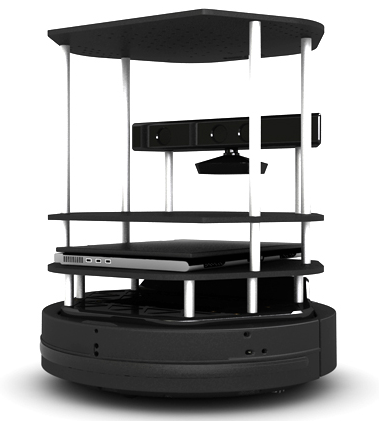
\includegraphics[width=0.3\columnwidth]{pictures/chapter10/turtlebot2.png}
\caption{Turtlebot2의 이미지}
\end{figure}

터틀봇은 매우 저렴한 가격이 가장 큰 무기로, TurtleBot 2의 기본 베이스인 Kobuki\footnote{http://garage.yujinrobot.com/robots/kobuki.html}\footnote{Kobuki 스팩과 이미지는 http://kobuki.yujinrobot.com/ 에서 공개한 정보를 기반으로 사용/재수정되어 작성 되었음을 밝힌다. 거북이 관련 문서/이미지 라이선스는 CC BY-SA 3.0 이다.} 의 경우 350 달러, TurtleBot 2 완제품 (도킹스테이션, 키넥트, 노트북, 폴과 스택등의 프레임 등)의 경우에는 1650달러에 판매되고 있다. TurtleBot 2 완제품의 경우 아래와 같은 사양으로 되어 있다.

%-------------------------------------------------------------------------------
\subsubsection{Hardware}

\begin{itemize}[leftmargin=*]
\item Kobuki Base (Yujinrobot )
\item Microsoft Kinect
\item Netbook (ROS Compatible)
\item Kinect Mounting Hardware (키넥트를 달 수 있는 기구)
\item TurtleBot Structure
\item TurtleBot Module Plate with 1 inch Spacing Hole Pattern (터틀봇 위에 노트북 등 다양한 디바이스를 장착하기 위한 프레임)
\end{itemize}

\noindent
개인적으로는, 터틀봇 본체, 토킹스테이션, 대용량 배터리, 스택 및 폴만을 구입하는것이 더 경제적이고, 키넥트 보다는 Asus Xtion 이 더 좋을 듯 싶다. 본 강좌에서는 기본 구성이 아닌 터틀봇 본체, 토킹스테이션, 대용량 배터리, 스택 및 폴, Xtion PRO LIVE, 노트북 혹은 인텔 NUC 의 구성된 하드웨어로 진행할 예정이다.

%-------------------------------------------------------------------------------
\subsubsection{Software}

\begin{itemize}[leftmargin=*]
\item 터틀봇 SDK
\item 데스크톱 개발 환경 (노트북의 경우)
\item visualization, planning, and perception, control and error handling 라이브러리
\item 데모 애플리케이션
\end{itemize}

이는 \url{https://github.com/turtlebot/turtlebot}에서 다운로드 가능하다.


%-------------------------------------------------------------------------------
\subsubsection{Open Source}
터틀봇은 오픈소스 소프트웨어 / 하드웨어 프로젝트로 진행되며, 아래의 라이센스를 갖고 있다.
Open Source Hardware Statement of Principles and Definition v1.0. 
FreeBSD Documentation License.

%-------------------------------------------------------------------------------
\section{Kobuki 하드웨어}\index{Kobuki 하드웨어}

%-------------------------------------------------------------------------------
\subsection{Kobuki \& Turtlebot2}\index{Kobuki}\index{turtlebot2}

Kobuki(거북이)는 유진로봇이 개발한 다목적 연구용 이동 로봇으로 나온 로봇 플랫폼이다. 이동 로봇 플랫폼이란 말 그대로 이동에 필요한 가장 기본이 되는 기능을 탑재한 제품으로 그 위에 사용자가 센서를 달아도 되고, 로봇암을 장착해도 되는 확장 가능 심플한 로봇 기반재라고 볼 수 있다. 그래서 그런지 거북이의 외관을 보면 매우 심플하다. 공학도들이 좋아하는 스타일이라고 볼 수 있다. 

이 로봇은 플랫폼이라는 명칭에 맞게 로봇 앞단에는 범퍼, 하단에는 절벽감지 센서, 바퀴 들림 센서, 고해상도 바퀴 엔코터, 모터, 3축 자이로 센서, 외부 디지털 입/출력 단자, 아날로그 입력 단자, 배터리까지 모두 포함된 완성품이다. 성능 또한 다년간 로봇 청소기을 개발/판매한 유진로봇답게 안정적이고 높은 신뢰도를 보인다. 

그리고, 거북이는 또 다른 이름이 있다. Turtlebot(터틀봇) 이라는 이름인데 이는 거북이를 기반으로 상위에 ROS를 탑재한 노트북PC, 3차원 정보를 취득하기 위해 Kinect 및 Xtion을 탑재한 또다른 종합 플랫폼이다. 터틀봇은 ROS 를 기반으로 한 연구소, 학교 등에서 많이 사용되고 있는 ROS의 공식적인 로봇이라고 볼 수 있다. 

ROS 중급 강좌를 위한 로봇 플랫폼으로서는 손색이 없다고 말할 수 있다. 단! 이 강좌를 작성하기 위하여 거북이 자료를 찾아 봤지만 관련 정보가 분산되어 있는 느낌이 강하다. 거북이는 하드웨어 및 소프트웨어는 완성도가 높지만 이 부분이 좀 아쉽다. 오픈소스 진영은 매뉴얼 및 사후관리는 힘들다는 것은 익히 알고 있지만 상용 제품으로서 정말 아쉬운 부분이라고 할 수 있다. 그래서 이번 강좌에서는 이 거북이에 대해서 집중 조명을 해볼 예정이다.

\begin{figure}[h]
\centering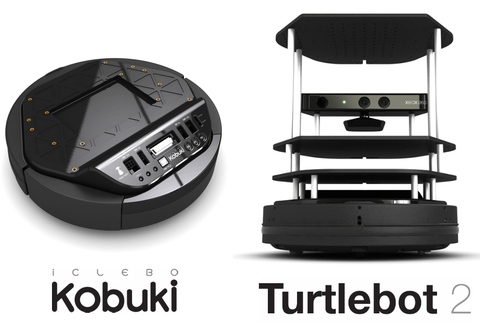
\includegraphics[width=0.5\columnwidth]{pictures/chapter10/kobuki_turtlebot2.png}
\caption{Kobuki와 Turtlebot2}
\end{figure}

%-------------------------------------------------------------------------------
\subsection{Kobuki 기본 구성}\index{Kobuki 기본 구성}

기본 구성은 1) 거북이 본체, 2) 리튬이온 배터리 (4S1P 14.6V 2200mAh), 3) USB 케이블, 4) 충전 어댑터, 그리고 5) 퀵 메뉴얼로 구성 되어 있다. 거기에 본 강좌의 시리즈에서는 충전소인 6) 도킹 스테이션과 장시간 구동을 위하여 7)리튬이온 배터리 (4S2P 14.6V 4400mAh) 를 추가 하기로 하겠다.

\begin{figure}[h]
\centering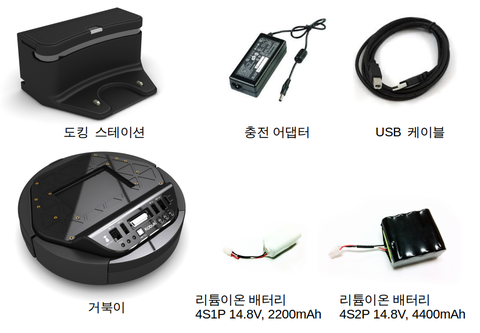
\includegraphics[width=0.7\columnwidth]{pictures/chapter10/kobuki_parts.png}
\caption{Kobuki 기본 구성품}
\end{figure}

%-------------------------------------------------------------------------------
\subsection{Kobuki 스펙}\index{Kobuki 스펙}

%-------------------------------------------------------------------------------
\subsubsection{모터 관련}\index{Kobuki 모터}

\begin{itemize}[leftmargin=*]
\item 모터 종류: Brushed DC Motor
\item 모터 제조사: Standard Motor
\item 모터 부품명: RP385-ST-2060
%\footnote{\url{http://www.standardmotor.net/sc_webcat/ecat/product_view.php\?lang\=1\&cat\=115&id=72\&page\=1}}
\end{itemize}

\begin{itemize}[leftmargin=*]
\item 드라이브 종류: 모터 양방향 구동용 전류 증폭 (H-bridge)
\item 제어 방식: Pulse-width modulation(PWM) 제어
\item 최대 직진 속도: 700 mm/s
\item 최대 회전 속도: 180 deg/s (※110 deg/s 보다 회전 속도가 높으면 자이로 성능이 떨어진다)
\item 최대 턱 극복 높이: 12 mm
\item 카펫 턱 극복 높이: 12 mm
\item 유효하중(Payload): 5 kg (일반), 4 kg (카펫위)
\end{itemize}

\begin{itemize}[leftmargin=*]
\item 정격전압(Rated Voltage): 12 V
\item 정격부하(Rated Load): 5 mN·m
\item 무부하 전류(No Load Current): 210 mA
\item 무부하 속도(No Load Speed): 9960 rpm ± 15\%
\item 정격부하 전류(Rated Load Current): 750 mA
\item 정격부하 속도(Rated Load Speed): 8800 rpm ± 15\%
\item 전기자 저항(Armature Resistance): 1.5506 Ω at 25°C
\item 전기자 인덕턴스(Armature Inductance): 1.51 mH
\item 토크 상수(Torque Constant(Kt)): 10.913 mN·m/A
\item 속도 상수(Velocity Constant(Kv)): 830 rpm/V
\item 스톨 전류(Stall Current): 6.1 A
\item 스톨 토크(Stall Torque): 33 mN·m
\end{itemize}

%-------------------------------------------------------------------------------
\subsubsection{센서 관련}\index{Kobuki 센서}

\begin{itemize}[leftmargin=*]
\item 주행기록계(Odometry) 센서: 52 ticks/enc rev, 2578.33 ticks/wheel rev, 11.7 ticks/mm
\item 3축 자이로(Gyro) 센서
: 공장 출하 시 캘리브레이션(calibration) 됨 (±20 deg/s to ±100 deg/s). 1축 정밀도 = 110 deg/s
  \begin{itemize}
  \item 제조사 : STMicroelectronics
  \item 제품명 : L3G4200D
  \item 측정범위 : ±250 deg/s
  \end{itemize}
\item 범퍼(Bumpers) 센서: 좌측, 중앙, 우측 / 총 3개
\item 클리프(Cliff) 센서: 좌측, 중앙, 우측 / 총 3개, (5cm 이상 감지될 경우 구동 정지)
\item 휠 드랍 (Wheel drop) 센서: 좌측, 우측 모터 부분 / 총 2개
\item 도킹(Docking) IR 수신기: 좌측, 중앙, 우측 / 총 3개
\item 모터 과부하 감지: 3A 이상의 전류가 흐릴 시 모터 작동이 중단됨
\item 센서 감지빈도(Sensor Data Rate): 50Hz
\end{itemize}

%-------------------------------------------------------------------------------
\subsubsection{전원 관련}\index{Kobuki 전원}

\begin{itemize}[leftmargin=*]
\item 배터리: 리튬 이온(Lithium-Ion), 14.8V, 2200 mAh (4S1P - 기본용량), 14.8V, 4400 mAh (4S2P - 대용량)
\item 배터리 모델: HYB ICR18650NH-2,200mAh\footnote{http://www.batteryspace.com/prod-specs/icr18650nh-2200.pdf}
\item 배터리 핀아웃
  \begin{itemize}
  \item Red: Battery (+), 9.6 V ~ 16.8 V
  \item White: NTC 온도센서 GND에 연결, 10 kΩ ± 1\%
  \item Black: Battery(-), Ground
  \end{itemize}
\item 최대 운영 시간: 3시간 (2200mAh), 7시간 (4400mAh)
\item 충전 시간: 1.5시간 (2200mAh), 2.6시간 (4400mAh)
\item 충전 어댑터(Recharging Adapter): 입력 전원=100-240V AC, 50/60Hz, 1.5A max; 출력=19V DC, 3.16A
\item 넷북 충전 커넥터(connector) : 19V/2.1A DC (단, 로봇이 충전중일 때)
\item 외부 장치로의 전원 공급 단자: 5V/1A, 12V/1.5A, 12V/5A (외부 장착 센서 및 보드에 전원 공급 가능)
\item 도킹 스테이션: 자율 충전 가능
\item 자율 충전 가능 공간: 충전 스테이션의 2미터 x 5미터 공간 이내
\end{itemize}

\begin{figure}[h]
\centering
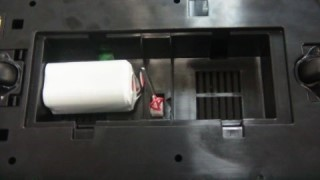
\includegraphics[width=0.4\columnwidth]{pictures/chapter10/battery1.jpg}
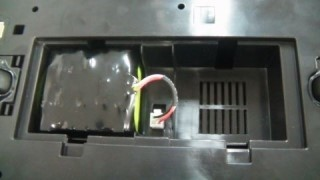
\includegraphics[width=0.4\columnwidth]{pictures/chapter10/battery2.jpg}
\caption{좌측: 리튬 이온 14.8V, 2200mAh를 연결한 경우, 우측: 리튬 이온 14.8V, 4400mAh를 연결한 경우}
\end{figure}

%-------------------------------------------------------------------------------
\subsubsection{기타}

\begin{itemize}[leftmargin=*]
\item 컴퓨터 연결 단자: USB 혹은 거북이 포트 내 있는 RX/TX 핀을 활용하여 가능
\item 확장 핀(Expansion pins): 
  \begin{itemize}
  \item 3.3V/1A 전원 공급 단자 1개
  \item 5V/1A  전원 공급 단자 1개
  \item 아날로그 입력 4 개 단자
  \item 디지털 입력 4개 단자
  \item 디지털 출력 4개 단자
  \end{itemize}
\item 오디오: 프로그래밍 가능한 비프음(beep) 소리
\item LED: 프로그래밍 가능한 2색 칼라 LED 2개 ({\color{limegreen}녹색},\textcolor{orange}{주황색},\textcolor{red}{적색} 표현이 가능)
\item 상태(State) 표기 LED: 2색 LED 1개 ({\color{limegreen}녹색}: 배터리 남은 잔량이 충분함, \textcolor{orange}{주황색}: 충전할 필요가 있음, {\color{limegreen}녹색 점멸} - 충전 중)
\item 버튼(Buttons): 3개의 터치 버튼
\item 펌웨어 업그레이드: 펌웨어 업그레이드 버튼을 설정한 후 USB 단자를 통해 업그레이드 됨 
\end{itemize}

%-------------------------------------------------------------------------------
\subsection{Kobuki 본체}\index{Kobuki 본체}

거북이에 대한 자세한 설명이 없다보니 처음 거북이를 이용하는 유저들에는 상당히 당혹 스러운 경우가 많을 것이다. 우선, 자신의 거북이의 각 부분을 아래의 그림과 맞추어 가며 모터, 센서, 단자 등이 어디에 위치해 있는가를 살펴두기로 하자. 이는 이어지는 강좌에서 프로그램시에 꼭 필요하다. 

\begin{figure}[h]
\centering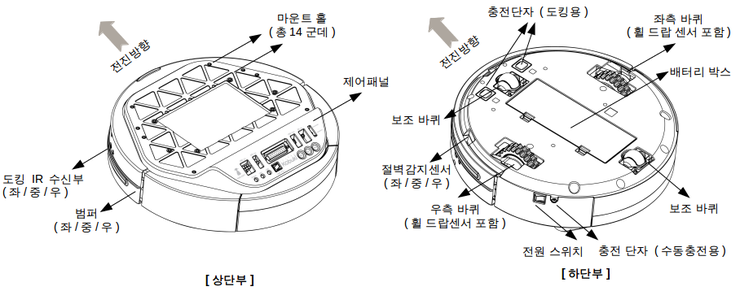
\includegraphics[width=0.9\columnwidth]{pictures/chapter10/kobuki_dimension.png}
\caption{Kobuki 본체의 각 부분의 설명}
\end{figure}

%-------------------------------------------------------------------------------
\subsection{Kobuki 제어패널}\index{Kobuki 제어패널}

거북이에는 제어패널이라고 하여 외부 센서 및 보드에 전원을 공급 가능하고 간단한 LED 및 버튼이 장착되어 있다. 각 부위에 대한 설명은 아래의 그림에 표시해 두었다.전원의 경우에는 랩탑(노트북), 임베디드 보드, Kinect, 범용용으로 4가지 외부 전원 공급을 할 수 있는 매우 편리한 기능을 가지고 있다. 자신만의 로봇을 제작할 경우, 이 전원핀을 사용하면 되겠다. 단, 각 전원핀인 아래의 커넥터를 이용하므로 참고하도록 하자. 개인적으로 거북이 구매시에 함께 구매하기를 강력 추천한다.

\begin{itemize}[leftmargin=*]
\item Molex PN : 43650-0218\footnote{\scriptsize\url{http://www.molex.com/molex/products/datasheet.jsp?part=active/0436500218_PCB_HEADERS.xml}} (5V,1A )
\item Molex PN : 43045-0224\footnote{\scriptsize\url{http://www.molex.com/molex/products/datasheet.jsp?part=active/0430450224_PCB_HEADERS.xml}} (12V,1.5A )
\item Molex PN : 5566-02B2\footnote{\scriptsize\url{http://www.molex.com/molex/products/datasheet.jsp?part=active/0039299022_PCB_HEADERS.xml}}  (12V,5A )
\item Molex PN : 3928-9068\footnote{\scriptsize\url{http://www.molex.com/molex/products/datasheet.jsp?part=active/0039289068_PCB_HEADERS.xml}}  (19V,2A )
\end{itemize}

\begin{figure}[h]
\centering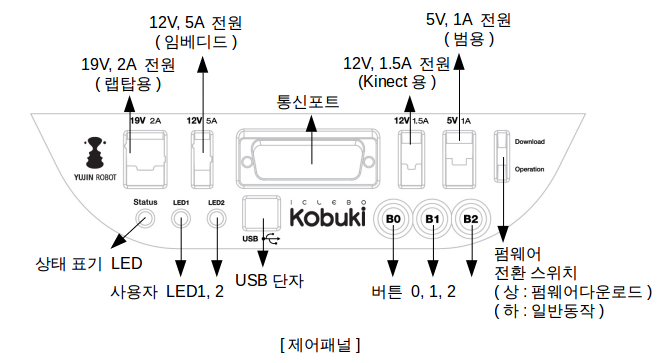
\includegraphics[width=0.8\columnwidth]{pictures/chapter10/kobuki_pannel.png}
\caption{Kobuki의 제어패널}
\end{figure}

\begin{figure}[h]
\centering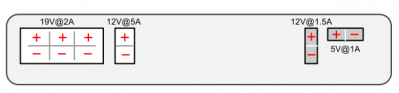
\includegraphics[width=0.6\columnwidth]{pictures/chapter10/kobuki_power.png}
\caption{Kobuki의 외부 전원}
\end{figure}

[참고사항] 
거북이의 상태 표기 LED
: 상태 표기 LED (Status LED)는 패널의 맨 왼쪽에 위치하고 있으며, 거북이의 현재 배터리 상태를 표기함
\begin{itemize}[leftmargin=*]
\item {\color{limegreen}녹색}: 기본 상태로 배터리가 충전되어 있음을 나타냄
\item \textcolor{orange}{주황색}: 배터리의 잔량이 낮은 상태를 나타냄 (충전이 필요한 상태임)
\item {\color{limegreen}녹색 점멸}: 배터리가 충전 중임을 나타냄
\end{itemize}

%-------------------------------------------------------------------------------
\subsection{Kobuki 통신 포트}\index{Kobuki 통신 포트}

%-------------------------------------------------------------------------------
\subsubsection{통신 포트의 각 핀의 설명}
거북이이는 통신, 디지털  입/출력, 아날로그 입력, 외부 전력 공급 등을 위하여 D-Sub25핀을 제공하고 있다. 제사한 사항은 각 핀의 명칭, 기능 등을 아래의 표에서 설명하고 있으니 참고하기 바란다.

\begin{figure}[h]
\centering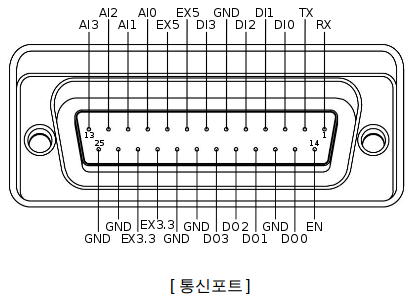
\includegraphics[width=0.5\columnwidth]{pictures/chapter10/kobuki_dsub25.png}
\caption{Kobuki의 D-Sub25 통신 포트}
\end{figure}

\begin{figure}[h]
\centering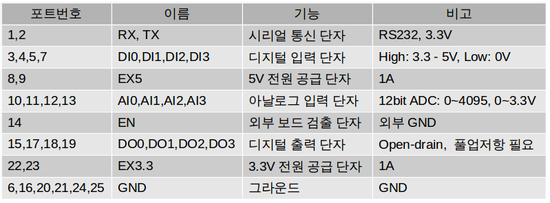
\includegraphics[width=0.8\columnwidth]{pictures/chapter10/kobuki_dsub25_num.png}
\caption{통신 포트의 각 핀의 설명}
\end{figure}

%-------------------------------------------------------------------------------
\subsubsection{SBC 및 MCU와의 연결}

거북이는 USB 를 연결을 통한 제어 이외에도 USB를 사용할 수 없는 SBC(Single Board Computer)와 MCU(Micro Control Unit)과도 시리얼 통신으로 연결하여 사용 가능하다. 그 방법을 아래에 소개한다.

\setcounter{num}{0}

\vspace{\baselineskip}
\noindent
\stepcounter{num}
\thenum) RS-232
거북이의 시리얼 포트의 사용 전압은 3.3V 이다. 최대 5V까지는 사용가능하지만 그 이상의 산업용 임베디트 리눅스 보드에서는 RS-232 방식으로 거북이와 연결하기 위해서는 통신 기준 전압을 맞추기 위하여 MAX232와 같은 라인 트랜시버 (line transceiver)를 경유해야 한다. 아래 사진 좌측의 경우.

\noindent
\stepcounter{num}
\thenum)) MCU와의 연결
거북이의 시리얼 핀의 입/출력은 3.3V ~ 5V 까지 허용되어 아래와 같이 직접 연결이 가능하다. 아래 사진 우측의 경우.

\noindent
\stepcounter{num}
\thenum) 통신 프로토콜
통신 프로토콜은 아래의 글을 참조하도록 하자.
\url{http://yujinrobot.github.io/kobuki/doxygen/enAppendixProtocolSpecification.html}

\begin{figure}[h]
\centering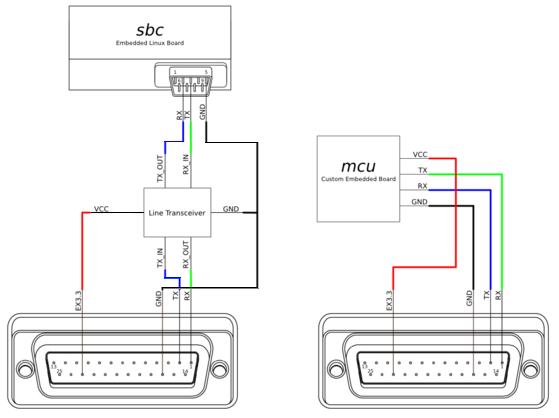
\includegraphics[width=0.9\columnwidth]{pictures/chapter10/kobuki_connect.png}
\caption{SBC 및 MCU와의 연결 방법}
\end{figure}

%-------------------------------------------------------------------------------
\subsubsection{통신포트 관련 회로도}

거북이의 통신포트와 관련하여 회로도를 제공하고 있다. 필요한 경우 링크\footnote{\url{http://kobuki.yujinrobot.com/files/5613/5526/9189/io_port_121024.pdf}}에서 다운로드 후 참고하도록 하자. 

%-------------------------------------------------------------------------------
\subsection{Kobuki 도킹 스테이션}

거북이이는 유저가 직접 충전 어댑터를 이용하여 본체에 연결하여 충전하는 기본 방식 이 외에 로봇이 스스로 충전소까지 이동하여 도킹 후 스스로 충전을 개시하는 "도킹 스테이션"을 제공한다. 독특한 점은 기본 구성품인 충전 어댑터를 도킹 스테이션에 끼워서 사용한다는 점이다. 재활용면에서 매우 실용적인 디자인이다. 이는 기본 구성 제품은 아니지만 매우 편리하고 도킹 방법에 대한 연구도 해볼 수 있어서 매우 유용해 보인다.

\noindent
[참고사항] 
도킹스테션의 상태 표기 LED: 충전 상태 표기 LED는 현재 충전 상태를 표기함
\begin{itemize}[leftmargin=*]
\item\textcolor{red}{적색}: 로봇이 도킹되어 있지 않은 상태
\item{\color{limegreen}녹색 점멸}: 로봇이 도킹되어 충전 중인 상태
\item{\color{limegreen}녹색}: 로봇이 도킹되어 있고, 충전이 완료된 상태
\end{itemize}

\begin{figure}[h]
\centering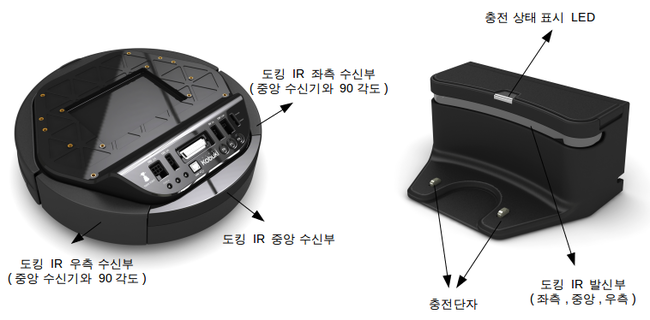
\includegraphics[width=0.8\columnwidth]{pictures/chapter10/kobuki_docking_station.png}
\caption{Kobuki 도킹 스테이션}
\end{figure}

%-------------------------------------------------------------------------------
\subsection{Kobuki 펌웨어 업데이트}

하드웨어 강좌에 걸맞지 않을지는 몰라도 처음 셋팅에 필요할듯 싶어 추가하였다. 업데이트와 관련하여 추가 설명이 많을 듯 싶어서 따로 강좌를 만들었다. "로봇 운영체제 강좌 : Kobuki의 펌웨어 업그레이드" 강좌를 참고하도록 하자.

%-------------------------------------------------------------------------------
\subsection{Kobuki 모델}

거북이의 2차원 및 3차원 모델은 각각 DWG, PDF 와 IGS, STEP, STL 으로 제공되고 있다. 모든 모델이 준비된 상황은 아니지만 플랫폼 위에 또 다른 기구나 센서를 추가할 경우 사용되는 거북이 치수 및 패널이 포함되어 있다.필요한 경우에는 아래의 링크의 모델을 참고하길 바란다.

\begin{itemize}[leftmargin=*]
\item 2차원 모델 : \url{http://files.yujinrobot.com/kobuki/hardware/drawings/}
\item 3차원 모델 : \url{http://files.yujinrobot.com/kobuki/hardware/models/}
\end{itemize}

%-------------------------------------------------------------------------------
\section{Kobuki 소프트웨어}\index{Kobuki 소프트웨어}

%-------------------------------------------------------------------------------
\subsection{Kobuki 관련 소프트웨어}

거북이 지원하는 소프트웨어는 크게 아래와 같이 3가지 분류된다. 1) SDK, 2) ROS, 3) OPRoS 가 있는데 우리는 이 강좌를 통해 다루는 것은 오직 ROS 용 소프트웨어를 가지고 거북이를 제어하도록 하겠다. ROS 지원 이외의 소프트웨어가 필요한 분들을 위하여 간략적인 정보를 아래에 담았다. 참고하기 바란다.

%-------------------------------------------------------------------------------
\subsubsection{SDK 지원 소프트웨어}

\setcounter{num}{0}

\vspace{\baselineskip}
\noindent
\stepcounter{num}
\thenum-1) 윈도우즈\\
: Windows, x86 컴퓨터, Visual Studio 2010 에서 작동가능한 소스를 제공한다.\\  
(\url{http://files.yujinrobot.com/kobuki/windows/sdk-kobuki-x86-vs10-release.zip})

\vspace{\baselineskip}
\noindent
\stepcounter{num}
\thenum-2) 리눅스 
: Linux, 캐킨(catkin) 기반으로 컴파일 가능한 환경을 제공한다.\\
(\url{https://github.com/yujinrobot/kobuki_core.git})

\vspace{\baselineskip}
\noindent
\stepcounter{num}
\thenum-3) 맥\\
: 공식적으로는 지원하지 않지만 리눅스용을 수정하면 가능할 듯 싶다. 또한, 아래와 같이 별도로 저장소를 제공하는 것을 보니 어렵지 않게 사용 가능 할 듯 싶다. 필자는 확인해보지는 않았지만 필요한 사람은 아래 링크의 저장소를 확인하도록 하자.\\
(\url{https://github.com/ros/homebrew-hydro})

\vspace{\baselineskip}
\noindent
\stepcounter{num}
\thenum-4) 임베디드\\
: MCU 에서 제어 가능하지만 자세한 정보는 찾아 볼 수 없다. "로봇 운영체제 강좌 : Kobuki의 하드웨어" 강좌에서 말한 시리얼 통신을 위한 통신 프로토콜을 참조하도록 하자.\\

윈도우즈, 리눅스, 맥, 임베디드를 위한 SDK에 대한 더 자세한 사항은 아래의 페이지를 참고하도록 하자.\\
Kobuki c++ library : \url{http://yujinrobot.github.io/kobuki/doxygen/enMainPage.html}

%-------------------------------------------------------------------------------
\subsubsection{ROS 지원 소프트웨어}

거북이는 별도의 플랫폼 없이도 각각의 OS 및 디바이스에 맞도록 개발된 SDK에 의하여 제어 가능하다. 하지만 플랫폼을 사용함으로써 더 다양한 기존 오픈소스 기반 소프트웨어를 사용할 수 있고, 자신의 소프트웨어 개발에도 큰 도움을 받게된다. 거북이는 개발 초기부터 ROS라는 플랫폼의 로봇 플랫폼으로서 개발되었다. 우리 오로카에서는 거북이의 ROS 기반 소프트웨어를 가지고 강좌를 진행할 것이다.
 
ROS 관련 소프트웨어는 크게 4 가지로 분류된다. kobuki 메타 패키지는 거북이 전반적인 소프트웨어가 모두 포함되어 있다. 우리가 주로 사용할 패키지들이 모두 이 안에 포함된다. 또 다른 메타 패키지로는 kobuki\_desktop 가 있다. 이는 가상 시뮬레이션 및 시각화와 관련된 패키지들을 모아둔 메타 패키지이다.그 이외에도 가상의 거북이를 RViz의 3차원 가식화 툴에서 구동해볼 수도 있으며, 순수 드라이버로 구성된 kobuki\_core 이라는 메타 패키지도 있다.

\setcounter{num}{0}

\vspace{\baselineskip}
\noindent
\stepcounter{num}
\thenum) kobuki 메타 패키지\\
위키: \url{http://wiki.ros.org/kobuki}\\
저장소: \url{https://github.com/yujinrobot/kobuki}\\
패키지: kobuki\_auto\_docking, kobuki\_bumper2pc, kobuki\_capabilities,\\
kobuki\_controller\_tutorial, kobuki\_description, kobuki\_keyop, kobuki\_node,\\
kobuki\_random\_walker, kobuki\_rapps, kobuki\_safety\_controller, kobuki\_testsuite

\vspace{\baselineskip}
\noindent
\stepcounter{num}
\thenum) kobuki\_desktop 메타 패키지\\
위키: \url{http://wiki.ros.org/kobuki_desktop}\\
저장소: \url{https://github.com/yujinrobot/kobuki_desktop}\\
패키지: kobuki\_dashboard, kobuki\_gazebo, kobuki\_gazebo\_plugins, kobuki\_qtestsuite

\vspace{\baselineskip}
\noindent
\stepcounter{num}
\thenum) kobuki\_soft 메타 패키지\\
위키: \url{http://wiki.ros.org/kobuki_soft}\\
저장소: \url{https://github.com/yujinrobot/kobuki_soft}\\
패키지: kobuki\_softapps, kobuki\_softnode

\vspace{\baselineskip}
\noindent
\stepcounter{num}
\thenum) kobuki\_core 메타 패키지\\
위키: \url{http://wiki.ros.org/kobuki_core}\\
저장소: \url{https://github.com/yujinrobot/kobuki_core}\\
패키지: kobuki\_dock\_drive, kobuki\_driver, kobuki\_ftdi

\vspace{\baselineskip}
\noindent
각 메타 패키지의 세부적인 내용 및 더 자세한 부가 설명은 다음 강좌에서 다루도록 하겠다.

%-------------------------------------------------------------------------------
\subsubsection{OPROS 지원 소프트웨어}

OPRoS 공식 홈페이지\footnote{\url{http://www.opros.or.kr/}}와 OPRoS 거북이 컴포넌트 페이지를 확인하기 바란다. Github 저장소는 다음과 같다.
\url{https://github.com/yujinrobot/kobuki_opros.git}

%-------------------------------------------------------------------------------
\section{Kobuki ROS 패키지}\index{Kobuki ROS 패키지}

%-------------------------------------------------------------------------------
\subsection{Kobuki 관련 메타 패키지}

거북이는 ROS 플랫폼을 사용함으로써 다양한 기존 오픈소스 기반 소프트웨어를 사용할 수 있고, 이것들을 이용하여 부가적으로 필요한 부분은 기존의 소프트웨어를 사용하고, 자신의 소프트웨어 개발에도 집중할 수 있게 된다. 

거북이의 ROS 관련 소프트웨어는 크게 4 가지로 분류된다. 하나는 kobuki 메타 패키지로 거북이 전반적인 소프트웨어가 모두 포함되어 있다. 우리가 주로 사용할 패키지들이 모두 이 안에 포함된다. 또 다른 메타 패키지로는 kobuki\_desktop 와 kobuki\_soft 가 있다. 이는 가상 시뮬레이션 및 시각화와 관련된 패키지들을 모아둔 메타 패키지이다. 그 이외에 순수 드라이버로 구성된 kobuki\_core 이라는 메타 패키지도 있다.

\begin{enumerate}
\item kobuki
\item kobuki\_desktop
\item kobkuki\_soft
\item kobuki\_core
\end{enumerate}

kobuki\_core는 순수한 기능의 드라이버를 포함한 메타 패키지 이다. 거북이 관련 하드웨어를 직접 다루기 위한 kobuki\_dock\_drive, kobuki\_driver, kobuki\_ftdi 가 포함되어 있지만 본 강좌에서는 다루지 않는다.

본 강좌에서는 ROS 지원 3 가지의 메타 패키지에 대해 간략히 알아보도록 하자.

\begin{definition}[메타패키지(metapackage)]
공통된 목적을 가지는 패키지들을 모아둔 패키지들의 집합을 말한다. 복수의 패키지를 포함하고 있다.
\end{definition}

%-------------------------------------------------------------------------------
\subsection{메타 패키지 kobuki 에 대한 간략한 설명}

\vspace{\baselineskip}
\begin{description}
\item[kobuki (메타 패키지)]
\item[위키]: \url{http://wiki.ros.org/kobuki}
\item[저장소]: \url{https://github.com/yujinrobot/kobuki}
\end{description}

\vspace{\baselineskip}
\noindent
ROS 지원 메타 패키지인 kobuki 패키지는 거북이 전반적인 소프트웨어가 모두 포함되어 있는 메타 패키지로 아래와 같은 패키지가 포함되어 있다. 우리가 주로 사용하게 될 패키지 들이니 한번 간단히 훑어 보기로 하자.

\setcounter{num}{0}

\vspace{\baselineskip}
\noindent\stepcounter{num}
\thenum) \textbf{kobuki\_node}
\begin{description}
\item[위키]: \url{http://wiki.ros.org/kobuki_node}
\item[기능]: 플랫폼 없이 사용가능한 순수한 거북이 구동 드라이버를 ROS용으로 재구성한 패키지이다. 또한 nodelet\footnote{nodelet은 같은 컴퓨터, 같은 프로세스에서 복수 알고리즘을 구동하기 위한 방법으로 ROS 에서 패키지 형태로 제공된다. 이는 네임스페이스를 이용하여 간단히 알고리즘 간의 복사 없이 재사용이 가능하고, 단/복수 스레드 기능을 API로 지원하고 있다.}을 기본 제공한다.
\end{description}

\vspace{\baselineskip}
\noindent\stepcounter{num}
\thenum) \textbf{kobuki\_keyop}
\begin{description}
\item[위키]: \url{http://wiki.ros.org/kobuki_keyop}
\item[기능]: 키보드로 거북이를 원격 조종하기 위한 패키지이다.
\end{description}

\vspace{\baselineskip}
\noindent\stepcounter{num}
\thenum) \textbf{kobuki\_random\_walker}
\begin{description}
\item[위키]: \url{http://wiki.ros.org/kobuki_random_walker}
\item[기능]: 거북이의 범퍼, 절벽, 휠 드랍 등의 센서를 이용하여 주위 환경을 탐색하며 돌아나니게 만들어둔 패키지이다. 거북이 동작 확인시에 도움이 되는 패키지이다.
\end{description}

\vspace{\baselineskip}
\noindent\stepcounter{num}
\thenum) \textbf{kobuki\_safety\_controller}
\begin{description}
\item[위키]: \url{http://wiki.ros.org/kobuki_safety_controller}
\item[기능]: 거북이 제어를 위한 컨트롤러가 주어지지만, 이는 안전을 고려하지 않은 상태이다. 그래서 거북이 사용상 안전을 위해서 이 패키지가 개발되었다. 즉, 각종 센서의 값을 이용하여 무리한 제어 및 사고를 미연에 방지해준다. 예를 들어 전진 명령을 내려도 전진 방향에 낭떠러지가 감지 되었을 경우에는 사용자의 명령을 무시하고 로봇을 정지하게 된다.
\end{description}

\vspace{\baselineskip}
\noindent\stepcounter{num}
\thenum) \textbf{kobuki\_controller\_tutorial}
\begin{description}
\item[위키]: \url{http://wiki.ros.org/kobuki_controller_tutorial}
\item[기능]: 거북이 제어를 위한 간단한 따라하기식 패키지이다. 거북이의 범퍼가 눌러졌을 경우, LED를 깜빡이는 기능을 담고 있다.
\end{description}

\vspace{\baselineskip}
\noindent\stepcounter{num}
\thenum) \textbf{kobuki\_description}
\begin{description}
\item[위키]: \url{http://wiki.ros.org/kobuki_description}
\item[기능]: 거북이의 시뮬레이션과 시각화를 위한 Urdf 모델을 담고 있다.
\end{description}

\vspace{\baselineskip}
\noindent\stepcounter{num}
\thenum) \textbf{kobuki\_auto\_docking}
\begin{description}
\item[위키]: \url{http://wiki.ros.org/kobuki_auto_docking}
\item[기능]: 거북이가 도킹 충전 스테이지에 도킹하여 충전하는 내용을 담을 패키지이다.
\end{description}

\vspace{\baselineskip}
\noindent\stepcounter{num}
\thenum) \textbf{kobuki\_bumper2pc}
\begin{description}
\item[위키]: \url{http://wiki.ros.org/kobuki_bumper2pc}
\item[기능]: 범퍼와 절벽센서를 점군(point cloud) 형태로 변환하는 내용을 담은 패키지이다. 이는 네비게이션에서 PC 데이터를 사용하고 있기에 이 패키지를 통해 이들의 정보도 네비게이션에서 사용할 수 있도록 돕고 있다.
\end{description}

\vspace{\baselineskip}
\noindent\stepcounter{num}
\thenum) \textbf{kobuki\_capabilities}
\begin{description}
\item[위키]: 없음
\item[기능]: 위키 페이지가 따로 없으며 패키지명만으로는 어떤 패키지인지 알 수 없다. 소스이라기 보다는 랍핑된 yaml 코드가 주를 이루고 있으며 실질적인 동작 노드가 있기 보다는 kobuki\_node 및 rocon\_apps 과 함께 동작하며 전체 패키지를 관리하는 수준의 패키지으로 보여진다.
\end{description}

\vspace{\baselineskip}
\noindent\stepcounter{num}
\thenum) \textbf{kobuki\_capabilities}
\begin{description}
\item[위키]: 없음
\item[기능]: 위키 페이지가 따로 없으며 패키지명만으로는 어떤 패키지인지 알 수 없다. 소스이라기 보다는 랍핑된 yaml 코드가 주를 이루고 있으며 실질적인 동작 노드가 있기 보다는 kobuki\_node 및 rocon\_apps 과 함께 동작하며 전체 패키지를 관리하는 수준의 패키지으로 보여진다.
\end{description}

\vspace{\baselineskip}
\noindent\stepcounter{num}
\thenum) \textbf{kobuki\_rapps}
\begin{description}
\item[위키]: 없음
\item[기능]: 위키등에 따로 설명이 없어서 정확히는 알 수 없지만, auto\_docking 와 random\_walker 를 실행 가능해 보이며, 안드로이드 앱에서 사용가능해 보인다.
\end{description}

\vspace{\baselineskip}
\noindent\stepcounter{num}
\thenum) \textbf{kobuki\_testsuite}
\begin{description}
\item[위키]: \url{http://wiki.ros.org/kobuki_testsuite}
\item[기능]: 거북이 하드웨어를 체크하기 위한 패키지이다. 각종 센서 값 및 로봇 구동을 테스트해 볼 수 있다.
\end{description}

%-------------------------------------------------------------------------------
\subsection{메타 패키지: kobuki\_desktop 에 대한 간략한 설명}

\vspace{\baselineskip}
\begin{description}
\item[kobuki\_desktop (메타 패키지)]
\item[위키]: \url{http://wiki.ros.org/kobuki_desktop}
\item[저장소]: \url{https://github.com/yujinrobot/kobuki_desktop}
\end{description}

\vspace{\baselineskip}
\noindent
ROS 지원 메타 패키지중 하나인 kobuki\_desktop 패키지는 거북이 관련 가상 시뮬레이션 및 시각화와 관련된 패키지들을 모아둔 메타 패키지로 아래와 같은 패키지가 포함되어 있다.

\setcounter{num}{0}

\vspace{\baselineskip}
\noindent\stepcounter{num}
\thenum) \textbf{kobuki\_dashboard}
\begin{description}
\item[위키]: \url{http://wiki.ros.org/kobuki_dashboard}
\item[기능]: RQT 베이스의 시각화를 위한 플러그인이다. 로봇 및 제어 PC의 배터리 정보, 에러, 경고 정보를 GUI 프로그램에서 확인할 수 있다.
\end{description}

\vspace{\baselineskip}
\noindent\stepcounter{num}
\thenum) \textbf{kobuki\_gazebo}
\begin{description}
\item[위키]: \url{http://wiki.ros.org/kobuki_gazebo}
\item[기능]: 3차원 시뮬레이션 Gazebo에서 거북이를 사용하기 위한 가상 시뮬레이션 관련 패키지이다.
\end{description}

\vspace{\baselineskip}
\noindent\stepcounter{num}
\thenum) \textbf{kobuki\_gazebo\_plugins}
\begin{description}
\item[위키]: \url{http://wiki.ros.org/kobuki_gazebo_plugins}
\item[기능]: kobuki\_gazebo와 함께 사용하는 패키지로 범퍼, 절벽, 오드메트리, IMU등의 센서를 이용가능하고, 거북이의 모터를 가상으로 제어할 수 있도록 해주는 패키지이다.
\end{description}

\vspace{\baselineskip}
\noindent\stepcounter{num}
\thenum) \textbf{kobuki\_qtestsuite}
\begin{description}
\item[위키]: \url{http://wiki.ros.org/kobuki_qtestsuite}
\item[기능]: RQT 의 하나의 플러그으로 거북이의 각종 테스트를 수행할 수 있게 도와주는 패키지이다. 공장에서 로봇 생명주기 테스트등이 포함되어 있는것을 보아 일반 유저용이라기 보다는 출하전 로봇 상태를 테스트하기 위한 용도로 사용되는 듯 싶다.
\end{description}

%-------------------------------------------------------------------------------
\subsection{메타 패키지: kobuki\_soft 에 대한 간략한 설명}

\vspace{\baselineskip}
\begin{description}
\item[kobuki\_soft (메타 패키지)]
\item[위키]: \url{http://wiki.ros.org/kobuki_soft}
\item[저장소]: \url{https://github.com/yujinrobot/kobuki_soft}
\end{description}

\vspace{\baselineskip}
\noindent
kobuki\_soft 는 많이 알려지지는 않았지만 ROS의 시각화툴인 RViz 환경에서 거북이의 동작을 시뮬레이션 할 수 있는 가상 시뮬레이션 환경을 제공해주는 패키지이다.

\setcounter{num}{0}

\vspace{\baselineskip}
\noindent\stepcounter{num}
\thenum) \textbf{kobuki\_softnode}
\begin{description}
\item[위키]: \url{http://wiki.ros.org/kobuki_softnode}
\item[기능]: 거북이 시뮬레이션과 관련된 가상 로봇 시뮬레이션 기능의 패키지이다. RViz 에서 실행 가능하다.
\end{description}

\vspace{\baselineskip}
\noindent\stepcounter{num}
\thenum) \textbf{kobuki\_softapps}
\begin{description}
\item[위키]: \url{http://wiki.ros.org/kobuki_softapps}
\item[기능]: kobuki\_softnode 와 연관되는 패키지로 시뮬레이션 관련 애플리케이션을 가지고 있으며 주로 네비게이션을 다루고 있다.
\end{description}

\vspace{\baselineskip}
\noindent
거북이의 하드웨어, 거북이 개발에 필요한 소프트웨어를 알아보고 우리가 사용하게 될 ROS 지원 패키지들에 대해서도 살펴보았다. 다음 강좌에서는 거북이를 실제로 동작해보며 위에서 소개한 패키지들에 대해서 하나하나 알아 나아가 보자.

%-------------------------------------------------------------------------------
\section{Kobuki 개발환경}\index{Kobuki 개발환경}

%-------------------------------------------------------------------------------
\subsection{로봇 초기 테스트}

거북이를 사용하기 위해서는 제어 컴퓨터에 리눅스 및 ROS 설치, 관련 패키지 설치까지 마치려면 상당한 시간이 필요하다. 개봉 후 로봇에 문제는 없는지 궁금하기 마련인데 거북이는 이러한 유저를 위하여 간단한 테스트 프로그램을 제어 컴퓨터 없이 실행가능하게 되어있다. 이를 함께 해보도록 하자. 

\setcounter{num}{0}

\vspace{\baselineskip}
\noindent\stepcounter{num}
\thenum) 거북이를 바닥의 안전한 위치에 둔다.\\
: (주의!) 책상 위 테이블 위는 피하도록 하자. 처음부터 대형 참사를 불러올 수 있다!

\vspace{\baselineskip}
\noindent\stepcounter{num}
\thenum) 거북이 전원 스위치를 킨다. 

\vspace{\baselineskip}
\noindent\stepcounter{num}
\thenum) 전원 스위치를 켠 후 3초 이내에 거북이 제어 패널의 B0 버튼을 2초간 눌렀다가 띤다.

\vspace{\baselineskip}
\noindent\stepcounter{num}
\thenum) 로봇이 자율적으로 움직이며 펌퍼에 장애물이 부딪쳤을 경우, 회전하고 다시 전진하게 된다.

\vspace{\baselineskip}
\noindent\stepcounter{num}
\thenum)  전원 스위치를 켠 후 3초 이내에 거북이 제어 패널의 B1 버튼을 2초간 눌렀다가 띤다.

\vspace{\baselineskip}
\noindent\stepcounter{num}
\thenum)  제어 패널의 B0 버튼을 누르면 앞으로 고속 전진한다.\\
: 매우 빠른속도로 돌진하게 된다. 주의 하도록 하자.

%-------------------------------------------------------------------------------
\subsection{개발환경}

본 강좌의 진행에 앞서서 필자의 개발 환경을 미리 알리고 시작하도록 하겠다. 꼭 반드시 동일할 필요는 없지만, 원할한 강좌 진행을 위해서는 아래와 같이 개발 환경을 권장한다. 이 이외에 환경에서의 질문에 대해서는 질응답은 하지만 실제 필자가 테스트해 볼 수 있는 상황이 아니기 때문에 대처하기 어려울 수도 있다. 필자의 소프트웨어 개발환경으로는 아래와 같다. ROS Indigo의 설치는 "로봇 운영체제 강좌 : Indigo 설치" 를 참고하기 바란다.

\begin{figure}[h]
\centering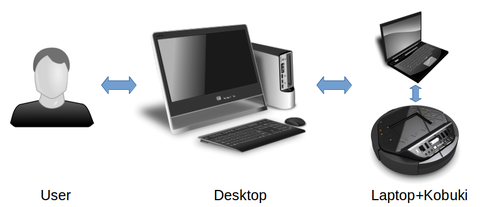
\includegraphics[width=0.8\columnwidth]{pictures/chapter10/develop_environment.png}
\caption{개발환경}
\end{figure}

%-------------------------------------------------------------------------------
\subsubsection{PC 1 (Desktop)}

\begin{itemize}[leftmargin=*]
\item Kobuki 조종, 외/내부 센서 데이터 처리, 네비게이션을 담당한다. 모든 개발은 이 컴퓨터에서 진행되게 된다.
\item Ubuntu 14.04 LTS 64bit (Trusty Tahr)
\item ROS - Indigo
\item ROS 패키지 : sudo apt-get install ros-indigo-kobuki* (거북이 관련 모든 패키지)
\end{itemize}

%-------------------------------------------------------------------------------
\subsubsection{PC 2 (Laptop)}

\begin{itemize}[leftmargin=*]
\item Kobuki 에 직접 탑재할 PC이며 직접적인 제어 및 센서 데이터를 받아 데스트톱으로 전송하게 된다.
\item Ubuntu 14.04 LTS 64bit (Trusty Tahr)
\item ROS - Indigo
\item 설치할 ROS 패키지 : ros-indigo-kobuki 와 ros-indigo-kobuki-core
 \end{itemize}

%-------------------------------------------------------------------------------
\subsection{거북이 패키지 설치하기}

앞으로의 강좌는 모두 데스크톱에서 진행할 예정이다. 다만, 거북이의 직접적인 제어 및 센서 데이터를 받아 데스크톱으로 전송하기 위하여 거북이용 랩톱에 거북이 관련 패키지를 설치하도록 하자. 아래의 설명은 랩톱과 데스크톱으로 나누어 설명하였으므로 참고하기 바란다.

%-------------------------------------------------------------------------------
\subsubsection{랩톱}

\setcounter{num}{0}

\vspace{\baselineskip}
\noindent\stepcounter{num}
\thenum) 랩톱에 "로봇 운영체제 강좌 : Indigo 설치" 를 참고하여 ROS Indigo 를 설치하자. 

\vspace{\baselineskip}
\noindent\stepcounter{num}
\thenum) "로봇 운영체제 강좌 : Indigo 설치" 의 "4. 환경 설정" 에서 랩톱의 경우에는 아래와 같이 설정하도록 하자. ROS\_MASTER\_URI 는 데스크톱의 IP를 와 ROS\_IP 에는 랩톱 자기 자신의  IP 로 설정해주도록 하자. 각각의 아이피는 새로운 터미널 창에서 ifconfig 명령어로 확인 할 수 있다.

\begin{lstlisting}[language=bash]
export ROS_MASTER_URI=http://%*데스크톱의아이피*):11311
export ROS_IP=%*랩톱의아이피*)
\end{lstlisting}

\vspace{\baselineskip}
\noindent\stepcounter{num}
\thenum) 다음과 같이 거북이의 직접적인 제어를 위한 필수 패키지를 설치하도록 하자.

\begin{lstlisting}[language=ROS]
sudo apt-get install ros-indigo-kobuki ros-indigo-kobuki-core
\end{lstlisting}

\vspace{\baselineskip}
\noindent\stepcounter{num}
\thenum) ROS 설치 이후 부터는 SSH(Secure Shell)를 이용하여 데스크톱에서 사용할 예정이기에  ssh를 설치하도록 하자.

\begin{lstlisting}[language=ROS]
sudo apt-get install ssh
\end{lstlisting}

%-------------------------------------------------------------------------------
\subsubsection{데스크톱}

\vspace{\baselineskip}
\noindent\stepcounter{num}
\thenum) 데스크톱에 "로봇 운영체제 강좌 : Indigo 설치" 를 참고하여 ROS Indigo 를 설치하자. 

\vspace{\baselineskip}
\noindent\stepcounter{num}
\thenum) "로봇 운영체제 강좌 : Indigo 설치" 의 "4. 환경 설정" 에서 데스크톱의 경우에는 ROS\_MASTER\_URI 와 ROS\_IP 모두 데스크톱의 IP로 설정해주도록 하자. 

\begin{lstlisting}[language=bash]
export ROS_MASTER_URI=http://%*데스크톱의아이피*):11311
export ROS_IP=%*데스크톱의아이피*)
\end{lstlisting}

\vspace{\baselineskip}
\noindent\stepcounter{num}
\thenum) 거북이 관련 모든 패키지를 설치하도록 하자. (시뮬레이션 관련은 추후에 추가로 설명한다.)

\begin{lstlisting}[language=ROS]
sudo apt-get install ros-indigo-kobuki*
\end{lstlisting}

\begin{corollary}[배보다 배꼽이 더 크다!]
터틀봇에 노트북을 하나 사용하는것은 정말 배보다 배꼽이 더 크게 느껴지는 분들이 있을 것이다. 노트북이 터틀봇 본체보다 비싸다는게 문제이다. 이 때에는 본 커뮤니티에서 라즈베리파이 및 오드로이드로 개발한 경험이 있으니 아래의 관련 글을 읽어보기 바란다. 단, Kinect, Xtion 등 Depth Camera 를 사용하기 위해서는 어느정도 고성능을 요구하기 때문에 라즈베리파이 보다는 오드로이드 정도의 최소 2.4GHz x 4코어 를 사용하기를 추천한다. 필자의 경우에는 앞서 말한바와 같이 범용적인 사용을 위하여 일반적으로 많이 사용하는 노트북과 같은 랩톱 환경에서 강좌를 진행할 예정이다. 
\end{corollary}

가장 기본적인 초기 테스트와 개발 환경 구축이 끝났다. 다음 강좌에서부터는 간단한 거북이 테스트를 수행하도록 하겠다.

%-------------------------------------------------------------------------------
\section{Kobuki 원격제어}\index{Kobuki 원격제어}

\setcounter{num}{0}

\vspace{\baselineskip}
\noindent\stepcounter{num}
\thenum) ROSCORE 구동\\
데스크톱에서 터미널창을 하나 열어, roscore 를 구동한다. 참고로 밑에서 설명하는 각 명령어는 각각 새로운 창을 열어 구동해줘야 한다.

\begin{lstlisting}[language=ROS]
roscore
\end{lstlisting}

\vspace{\baselineskip}
\noindent\stepcounter{num}
\thenum) SSH를 이용한 데스크톱에서 랩톱 접속하기\\
거북이와 랩톱을 usb 케이블로 연결 후에 전원 스위치를 켜준다. 그 후, 데스크톱에서 ssh 로 랩톱에 접속한다. 예를 들어, 터미널에서 " ssh kobuki@192.168.4.21 " 와 같이 입력해주면 랩톱에 연결할 수 있고, 쉘 명령어로 제어 가능하다.

\begin{lstlisting}[language=ROS]
ssh %*유저명@랩톱의아이피*)
\end{lstlisting}

\vspace{\baselineskip}
\noindent\stepcounter{num}
\thenum) 거북이 포트 생성\\
랩톱에 전속된 후, 아래와 같이 create\_udev\_rules 노드를 실행해 주면 /dev/kobuki 포트가 생성된다. 

\begin{lstlisting}[language=ROS]
rosrun kobuki_ftdi create_udev_rules
\end{lstlisting}

실행후, usb 케이블을 연결 해제 후에 다시 꼽아 주도록 하자. 그러면 ls -l 명령어로 해당 포트를 확인할 수 있다.

\begin{lstlisting}[language=ROS]
ls -l /dev/kobuki
lrwxrwxrwx 1 root root 7 Aug 24 14:26 /dev/kobuki -> ttyUSB0
\end{lstlisting}

필자의 경우, /dev/kobuki 의 포트는 본래 ttyUSB0 로 링크되어 있다는 것을 확인할 수 있다. ttyUSB0,1,2 등과 같이 연결 상황에 따라 달라지는 것을 create\_udev\_rules 노드를 통해 /dev/kobuki 이라는 통일된 포트로 사용할 수 있도록 돕고 있다.

\vspace{\baselineskip}
\noindent\stepcounter{num}
\thenum) 거북이 구동\\
아래의 명령어를 구동학 되면 비프음으로 소리가 나며, 초기 설정을 마친 후 거북이는 구동 상태로 바뀐다. 랩톱에서 실행해야하는 노드는 이것이 전부이다. 종료는 Ctrl + c 를 이용하면 된다. SSH 사용은 이것으로 마무리 되었다.

\begin{lstlisting}[language=ROS]
roslaunch kobuki_node minimal.launch
\end{lstlisting}

\vspace{\baselineskip}
\noindent
참고로, 아래와 같이 --screen 옵션을 붙여주게 되면 구동시에 발생되는 일부 숨겨진 메시지들까지 모두 확인할 수 있다. 거북이 사용중 원인 모를 에러가 있을 경우에는 아래처럼 --screen 옵션으로 확인해 보자. 참고로, 필자는 항상 --screen 옵션을 붙여주고 실행한다.

\begin{lstlisting}[language=ROS]
roslaunch kobuki_node minimal.launch --screen 
\end{lstlisting}

\vspace{\baselineskip}
\noindent\stepcounter{num}
\thenum) 키보드 제어 노드 구동\\
데스크톱에서 아래와 같이 명령어를 입력해주면 거북이를 원격 제어 할 수 있는 상태가 된다. 사용가능한 키는 밑에 정리해두겠다. 범퍼가 장착되어 있는 부분이 로봇의 앞 부분으로 전진 방향에 주의하도록 하자. 아래에 전진 방향의 그림을 첨부하니 참고하기 바란다.

\begin{lstlisting}[language=ROS]
roslaunch kobuki_keyop keyop.launch
\end{lstlisting}

\begin{itemize}[leftmargin=*]
\item 방향키 ↑ : 리니어 속도 지정으로 전진 방향으로 이동한다. (0.5씩, 단위 = m/sec) 
\item 방향키 ↓ : 리니어 속도 지정으로 후진 방향으로 이동한다. (0.5씩, 단위 = m/sec) 
\item 방향키 ← : 회전 속도 지정으로 시계 반대 방향으로 회전한다. (0.33씩, 단위 = rad/sec) 
\item 방향키 → : 회전 속도 지정으로 시계 방향으로 회전한다. (0.33씩, 단위 = rad/sec) 
\item 스페이스바 : 리니어 속도 및 회전 속도를 초기화 한다.
\item d : 모터를 비활성화 한다. (구동 불가능 상태)
\item e : 모터를 활성화 한다. (구동 가능 상태)
\item q : 종료
\end{itemize}

\begin{figure}[h]
\centering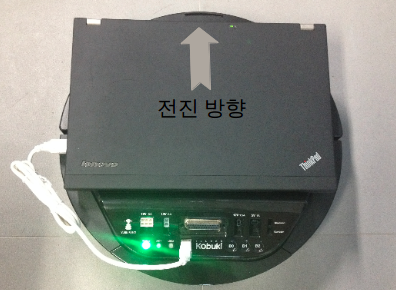
\includegraphics[width=0.7\columnwidth]{pictures/chapter10/kobuki_test.png}
\caption{Kobuki의 전진 방향}
\end{figure}

\vspace{\baselineskip}
\noindent
참고로, 아래와 같이 "safe\_keyop.launch" 으로 실행할 경우, 과도한 속도 변화 및 범퍼, 절벽감지, 휠 드랍 센서등의 반응에 따라 위험한 상황을 피할 수 있게 하는 방법도 있다. 또한, 속도를 급변하게 변화시키는 것이 아닌 부드러운 변화 곡선을 만들어서 원격 제어시에 속도 변화가 있더라도 부드럽게 구동 이동키실 수 있다. 사용자의 작은 실수로 로봇이 손상되는 것을 막기 위함이기 때문에 이러한 상황이 요구된다면 아래의 방법을 권장하는 바이다.

\begin{lstlisting}[language=ROS]
roslaunch kobuki_keyop safe_keyop.launch
\end{lstlisting}

전 강좌와 이번 강좌로 가장 기본적인 개발 환경 구축 및 테스트가 끝났다. 다음 강좌에서부터는 이전에 소개한 거북이 관련 패키지의 노드들을 하나하나 직접 구동해보는 시간을 갖도록 하겠다.

%-------------------------------------------------------------------------------
\section{Kobuki 토픽(Topic)}\index{Kobuki 토픽(Topic)}

%-------------------------------------------------------------------------------
\subsection{거북이 노드의 토픽}

우선, "로봇 운영체제 강좌 : Kobuki 구동 테스트" 의 글에서 처럼 "roslaunch kobuki\_node minimal.launch" 으로 거북이를 구동시켜 주자. 거북이를 구동시키게 되면 kobuki\_node 노드가 작동되고 거북이의 범퍼, 절벽, 들림센서, 모터 구동부 등이 토픽 형태로 발행 및 수신하게 된다.  오늘은 이 토픽들을 확인해 볼 예정이다.

데스크톱에서 거북이를 포함하여 아무런 노드가 실행하지 않은 상태에서 roscore만을 구동시킨 상태라면 "rostopic list" 으로 토픽 리스트를 살펴봐도 /rosout, /rosout\_agg 밖에 나오지 않는다. 하지만 위와 같이 kobuki\_node 를 실행하게 되면 아래와 같이 kobuki\_node에서 사용되는 다양한 토픽들을 확인할 수 있다.

\begin{lstlisting}[language=ROS]
$ rostopic list
/diagnostics
/diagnostics_agg
/diagnostics_toplevel_state
/joint_states
/mobile_base/commands/controller_info
/mobile_base/commands/digital_output
/mobile_base/commands/external_power
/mobile_base/commands/led1
/mobile_base/commands/led2
/mobile_base/commands/motor_power
/mobile_base/commands/reset_odometry
/mobile_base/commands/sound
/mobile_base/commands/velocity
/mobile_base/controller_info
/mobile_base/debug/raw_control_command
/mobile_base/debug/raw_data_command
/mobile_base/debug/raw_data_stream
/mobile_base/events/bumper
/mobile_base/events/button
/mobile_base/events/cliff
/mobile_base/events/digital_input
/mobile_base/events/power_system
/mobile_base/events/robot_state
/mobile_base/events/wheel_drop
/mobile_base/sensors/core
/mobile_base/sensors/dock_ir
/mobile_base/sensors/imu_data
/mobile_base/sensors/imu_data_raw
/mobile_base/version_info
/mobile_base_nodelet_manager/bond
/odom
/rosout
/rosout_agg
/tf
\end{lstlisting}

또한, GUI로 확인하고자 하는 경우에는 아래의 명령어로 전체의 실행된 노드 및 토픽들을 확인해 볼 수 있다. Node Graph의 초기설정에서 dead sinks 및 leaf topics 들은 안보이게 설정되어 있으니 아래의 그림을 참조하여 모든 토픽을 확인해보자.

\begin{lstlisting}[language=ROS]
$ rqt_graph
\end{lstlisting}

\begin{figure}[h]
\centering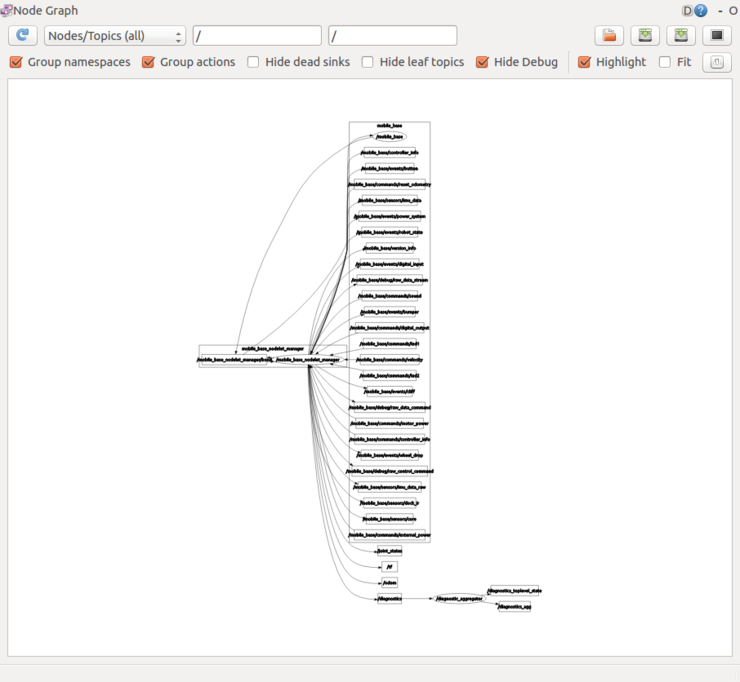
\includegraphics[width=0.5\columnwidth]{pictures/chapter10/rqt_graph_kobuki.png}
\caption{Kobuki의 노드 전개 상황}
\end{figure}

%-------------------------------------------------------------------------------
\subsection{수신 토픽}

위에서 언급한 토픽은 거북이 자기 자신이 수신받는 수신 토픽(Subscribed Topic)와 직접 발행하는 발행 토픽(Published Topic)으로 나눌 수 있다. 그 중 수신 토픽은 아래와 같다.

\begin{lstlisting}[language=ROS]
/mobile_base/commands/controller_info
/mobile_base/commands/digital_output
/mobile_base/commands/external_power
/mobile_base/commands/led1
/mobile_base/commands/led2
/mobile_base/commands/motor_power
/mobile_base/commands/reset_odometry
/mobile_base/commands/sound
/mobile_base/commands/velocity
\end{lstlisting}

각각의 수신 토픽에 대한 자세한 설명은 아래와 같다. 모든 수신 토픽을 알아둘 필요는 없지만 몇가지 테스트를 통해 사용하는 방법을 알아보도록 하자. 다른 것은 제외 하더라도 velocity 은 꼭 알아두도록 하자. velocity 는 로봇을 제어하는 실질적인 토픽으로 사용자는 로봇의 전/후진 및 좌/우 회전등의 제어를 이 토픽을 통해 실현할 수 있다.

\vspace{\baselineskip}
\begin{description}
\item[이름]: controller\_info 
\item[형태]: kobuki\_msgs/ControllerInfo
\item[기능]: PID 게인 설정 (기본값 PID Gain: Kp=100, Ki=0.1, Kd=2)
\end{description}

\vspace{\baselineskip}
\begin{description}
\item[이름]: digital\_output 
\item[형태]: kobuki\_msgs/DigitalOutput
\item[기능]: 디지털 출력 핀 제어
\end{description}

\vspace{\baselineskip}
\begin{description}
\item[이름]: external\_power
\item[형태]: kobuki\_msgs/ExternalPower
\item[기능]: 외부 전원의 On/Off
\end{description}

\vspace{\baselineskip}
\begin{description}
\item[이름]: led1
\item[형태]: kobuki\_msgs/Led
\item[기능]: LED1 제어
\end{description}

\vspace{\baselineskip}
\begin{description}
\item[이름]: led2
\item[형태]: kobuki\_msgs/Led
\item[기능]: LED2 제어
\end{description}

\vspace{\baselineskip}
\begin{description}
\item[이름]: motor\_power
\item[형태]: kobuki\_msgs/MotorPower
\item[기능]: 거북이 모터의 On/Off
\end{description}

\vspace{\baselineskip}
\begin{description}
\item[이름]: reset\_odometry
\item[형태]: std\_msgs/Empty
\item[기능]: 오도메트리(odometry) 리셋
\end{description}

\vspace{\baselineskip}
\begin{description}
\item[이름]: sound
\item[형태]: kobuki\_msgs/Sound
\item[기능]: 비프음 소리 출력
\end{description}

\vspace{\baselineskip}
\begin{description}
\item[이름]: velocity
\item[형태]: geometry\_msgs/Twist
\item[기능]: 로봇 전/후진,회전 제어, 속도 m/s, rad/s (실질적인 로봇 구동 제어)
\end{description}

%-------------------------------------------------------------------------------
\subsection{수신 토픽을 이용한 로봇 제어}

위에서 언급한 수신 토픽은 사용자가 발행한 토픽을 로봇이 받아 처리하게 되어 있다. 모든 토픽을 해보기에는 강좌가 길어지기 때문에 몇 가지 수신 토픽을 예를 들어 사용해보도록 하겠다.

\subsubsection{LED1 제어}
아래의 명령어로 거북이의 제어패널에 위치한 LED1의 불이 켜지게 된다. value은 0,1,2,3 까지 설정 가능하다. 0은 LED 를 끄게 되고, 1은 녹색, 2는 주황색, 3은 빨간색이 켜지게 된다.

\begin{lstlisting}[language=ROS]
rostopic pub /mobile_base/commands/led1 kobuki_msgs/Led "value: 1"
\end{lstlisting}


\subsubsection{비프음 제어}
아래의 명령어로 거북이의 비프임을 제어 가능하다. 옵션인 value은 0부터 6까지 7가지의 설정이 가능하다. 

\begin{description}
\item[0] - 전원 On 소리
\item[2] - 충전 시작  소리
\item[3] - 버튼 클릭 소리
\item[4] - 에러 발생 소리
\item[5] - 청소 시작 소리
\item[6] - 청소 종료 소리
\end{description}

\begin{lstlisting}[language=ROS]
rostopic pub /mobile_base/commands/sound kobuki_msgs/Sound "value: 6"
\end{lstlisting}


\subsubsection{속도 제어}

아래의 명령어로 거북이를 직접 구동할 수 있다. 여기서 사용되는 x, y 방향으로의 속도의 단위는 ROS 표준인 m/s 이고, z의 경우에는 rad/s 이다. 

\vspace{\baselineskip}
\begin{lstlisting}[language=ROS]
rostopic pub /mobile_base/commands/velocity geometry_msgs/Twist "linear:
  x: 0.2
  y: 0.0
  z: 0.0
angular:
  x: 0.0
  y: 0.0
  z: 0.0"
\end{lstlisting}

\begin{lstlisting}[language=ROS]
rostopic pub /mobile_base/commands/velocity geometry_msgs/Twist "linear:
  x: 0.0
  y: 0.0
  z: 0.0
angular:
  x: 0.0
  y: 0.0
  z: 1.0"
\end{lstlisting}

%-------------------------------------------------------------------------------
\subsection{발행 토픽}

거북이가 직접 발행하는 발행 토픽(Published Topic)은 아래와 같다. 크게 나누어 상태 진단(diagnostics) 관련 토픽, 디버그 관련 토픽, 이벤트 관련 토픽, 센서 관련 토픽으로 나눌 수 있으며 그 이외에 조인트 관련 토픽(joint\_states), 컨트롤 정보관련 토픽(controller\_info), 오드메트리(odom) 및 변환(tf) 관련 토픽 등이 있다.

\begin{lstlisting}[language=ROS]
/diagnostics
/diagnostics_agg
/diagnostics_toplevel_state
/joint_states
/mobile_base/controller_info
/mobile_base/debug/raw_control_command
/mobile_base/debug/raw_data_command
/mobile_base/debug/raw_data_stream
/mobile_base/events/bumper
/mobile_base/events/button
/mobile_base/events/cliff
/mobile_base/events/digital_input
/mobile_base/events/power_system
/mobile_base/events/robot_state
/mobile_base/events/wheel_drop
/mobile_base/sensors/core
/mobile_base/sensors/dock_ir
/mobile_base/sensors/imu_data
/mobile_base/sensors/imu_data_raw
/mobile_base/version_info
/mobile_base_nodelet_manager/bond
/odom
/tf
\end{lstlisting}

각각의 발행 토픽에 대한 자세한 설명은 아래와 같다. 모든 발행 토픽을 알아둘 필요는 없지만 몇가지 테스트를 통해 사용하는 방법을 알아보도록 하자. 특히, 오도메트리 정보를 담고 있는 odom, 변환 정보 인 tf, 조인트 정보 joint\_states 및 센서 관련 정보들은 앞으로의 거북이 사용에서 필수적으로 사용하는 토픽들이니 어떤 정보를 담고 있는지 꼭 알아두기 바란다.

%-------------------------------------------------------------------------------
\subsubsection{이벤트 관련}

\vspace{\baselineskip}
\begin{description}
\item[이름]: bumper
\item[형태]: kobuki\_msgs/BumperEvent
\item[기능]: 범퍼의 On/Off 이벤트, 좌측(0), 중앙(1), 우측(2)의 범퍼 상태를 나타내며, 보통 상태가 0, 눌렀을 경우 1이다.
\end{description}

\vspace{\baselineskip}
\begin{description}
\item[이름]: button
\item[형태]: kobuki\_msgs/ButtonEvent
\item[기능]: 버튼의 On/Off 이벤트, 버튼 0,1,2 의 값으로 보통 상태가 0, 눌렀을 경우 1이다.
\end{description}

\vspace{\baselineskip}
\begin{description}
\item[이름]: cliff
\item[형태]: kobuki\_msgs/CliffEvent
\item[기능]: 절벽 감지 센서의 이벤트, 좌측(0), 중앙(1), 우측(2)의 절벽 감지 상태를 나타내며, 보통 상태가 0, 절벽으로 판단될 경우 1이다. 이는 거리 센서 계측 값으로 결정되며, 절벽과 주행하고 있는 바닥과의 거리가 출력된다. 이 거리는 ROS 표준인 m 단위가 아닌듯 싶다. 제조사에 확인할 필요가 있음.
\end{description}

\vspace{\baselineskip}
\begin{description}
\item[이름]: digital\_input
\item[형태]: kobuki\_msgs/DigitalInputEvent
\item[기능]: 디지털 입력값(DI0,1,2,3)이 변화되었을 때 사용 가능하다. 즉, 이용하면 MCU 등이 없어도 추가적인 스위치 등에 사용할 수 있다.
\end{description}

\vspace{\baselineskip}
\begin{description}
\item[이름]: power\_system
\item[형태]: kobuki\_msgs/PowerSystemEvent
\item[기능]: 전원 상태를 나타낸다. 언플러그, 어댑터 및 도킹 스테이션에 연결된 상태인지 등, 총 6개의 상태를 표시 가능한다. 배터리가 매우 적은 상태인 4번 등이 이벤트로 발생될 경우, 도킹 충전 스테이지를 찾아서 자동 충전등에 이용하면 좋을 듯 싶다.\\
0 = UNPLUGGED\\
1 = PLUGGED\_TO\_ADAPTER\\
2 = PLUGGED\_TO\_DOCKBASE\\
3 = CHARGE\_COMPLETED\\
4 = BATTERY\_LOW\\
5 = BATTERY\_CRITICAL
\end{description}

\vspace{\baselineskip}
\begin{description}
\item[이름]: robot\_state
\item[형태]: kobuki\_msgs/RobotStateEvent
\item[기능]: 로봇의 온라인/오프라인의 상태를 표시해 준다고는 하는데 오프라인이 어떤 의미인지는 파악이 안된다.
\end{description}

\vspace{\baselineskip}
\begin{description}
\item[이름]: wheel\_drop
\item[형태]: kobuki\_msgs/WheelDropEvent
\item[기능]: 좌측(0), 우측(1)의 바퀴가 들렸는지에 대한 휠 드랍 상태를 나타내며, 보통 상태가 0, 바퀴가 들렸을 경우 1이다. 
\end{description}

%-------------------------------------------------------------------------------
\subsubsection{센서 관련}

\vspace{\baselineskip}
\begin{description}
\item[이름]: core
\item[형태]: kobuki\_msgs/SensorState
\item[기능]: 50Hz 주기로 제어에 필요한 거의 모든 센서의 값을 확인할 수 있는 토픽이다. 확인 할 수 있는 데이터는 bumper, wheel\_drop, cliff, left\_encoder, right\_encoder, left\_pwm, right\_pwm, buttons, charger, battery, bottom, current, over\_current, digital\_input, analog\_input 이다. 각 데이터의 단위는 kobuki\_msgs/SensorState\footnote{\url{http://docs.ros.org/indigo/api/kobuki_msgs/html/msg/SensorState.html}} 를 참고하자. 
\end{description}

\vspace{\baselineskip}
\begin{description}
\item[이름]: dock\_ir
\item[형태]: kobuki\_msgs/DockInfraRed
\item[기능]: 도킹 충전 스테이지에서 주사하고 있는 적외선 LED을 거북이가 수신했을때 아래와 같이 근접값으로 바꾸어 표시하고 있다.\\
NONE  =  0\\
NEAR\_LEFT =  1\\
NEAR\_CENTER =  2\\
NEAR\_RIGHT =  4\\
FAR\_LEFT = 16\\
FAR\_CENTER  =  8\\
FAR\_RIGHT = 32
\end{description}

\vspace{\baselineskip}
\begin{description}
\item[이름]: imu\_data
\item[형태]: sensor\_msgs/Imu
\item[기능]: 자이로 센서의 데이터로 방향과 z축의 각속도 정보를 나타낸다.
\end{description}

\vspace{\baselineskip}
\begin{description}
\item[이름]: imu\_data\_raw
\item[형태]: sensor\_msgs/Imu
\item[기능]: 자이로 센서의 가공 전 데이터로 x, y, z 축의 각속도 데이터를 나타낸다.이를 가공한 정보가 위에서 설명한 imu\_data 토픽이다.
\end{description}

%-------------------------------------------------------------------------------
\subsubsection{디버그 관련}

\vspace{\baselineskip}
\begin{description}
\item[이름]: raw\_control\_command
\item[형태]: std\_msgs/Int16MultiArray
\item[기능]: 디버깅용, 속도 제어 명령어인 두개의 속도 명령어의 송/수신 값을 확인 할 수 있다.
\end{description}

\vspace{\baselineskip}
\begin{description}
\item[이름]: raw\_data\_command
\item[형태]: std\_msgs/String
\item[기능]: 디버깅용, 로봇에게 송신한 가공 전 바이트 스트림 값을 확인할 수 있다.
\end{description}

\vspace{\baselineskip}
\begin{description}
\item[이름]: raw\_data\_stream
\item[형태]: std\_msgs/String
\item[기능]: 디버깅용, 로봇으로부터 수신 받은 가공 전 바이트 스트림 값을 확인할 수 있다.
\end{description}

%-------------------------------------------------------------------------------
\subsubsection{기타 관련}

\vspace{\baselineskip}
\begin{description}
\item[이름]: odom
\item[형태]: nav\_msgs/Odometry
\item[기능]: ★★★ 자이로와 엔터더 정보를 기반으로한 거북이의 오도메트리 정보를 얻을 수 있다. 네비게이션에 필요한 정보이니 꼭 알아두도록 하자.
\end{description}

\vspace{\baselineskip}
\begin{description}
\item[이름]: tf
\item[형태]: tf2\_msgs/TFMessage
\item[기능]: base\_footprint 와 odom 위치의 변환값을 가지고 있다.
\end{description}

\vspace{\baselineskip}
\begin{description}
\item[이름]: joint\_states
\item[형태]: sensor\_msgs/JointState
\item[기능]: 좌/우측 바퀴를 조인트로 여겼을 때의 위치, 속도, 힘 등을 확인 가능하다. 각 단위는 위치의 경우 m, 속도의 경우 m/s, 돌림힘의 경우 N·m 이다.
\end{description}

\vspace{\baselineskip}
\begin{description}
\item[이름]: diagnostics
\item[형태]: diagnostic\_msgs/DiagnosticArray
\item[기능]: 1Hz 주기로 자기 진단 정보를 얻을 수 있다.
\end{description}

\vspace{\baselineskip}
\begin{description}
\item[이름]: version\_info
\item[형태]: kobuki\_msgs/VersionInfo
\item[기능]: 거북이의 하드웨어, 펌웨어, 소프트웨어의 등의 정보를 얻을 수 있다. 참고로 필자가 소유하고 있는 버전의 경우 아래와 같다. (최신 펌웨어 업데이트를 한 경우임)\\
hardware: 1.0.4\\
firmware: 1.2.0\\
software: 0.6.0
\end{description}

%-------------------------------------------------------------------------------
\subsection{발행 토픽을 통해 로봇 상태 파악}

위에서 언급한 발행 토픽은 로봇의 센서값, 모터 상태, 로봇의 위치 등의 정보를 담아 토픽 형태로 전송하게 된다.아래에서는 일부 토픽을 수신하고 현재 로봇 상태를 알아보도록 하자.

\setcounter{num}{0}

\vspace{\baselineskip}
\noindent
\stepcounter{num}
\thenum) 범퍼 값 확인\\
좌측(0), 중앙(1), 우측(2)의 범퍼 상태를 나타내며, 보통 상태가 0, 눌렀을 경우가 1로 표시되는 것을 확인 할 수 있다.

\vspace{\baselineskip}
\begin{lstlisting}[language=ROS]
$ rostopic echo /mobile_base/events/bumper
---
bumper: 1
state: 1
---
bumper: 1
state: 0
---
\end{lstlisting}

\vspace{\baselineskip}
\noindent
\stepcounter{num}
\thenum) 센서
50Hz 주기로 제어에 필요한 거의 모든 센서의 값을 확인 할 수 있는 토픽이다. 각 센서의 데이터 단위는 kobuki\_msgs/SensorState에서 확인하도록 하자.

\vspace{\baselineskip}
\begin{lstlisting}[language=ROS]
$ rostopic echo /mobile_base/sensors/core
---
header: 
  seq: 357
  stamp: 
    secs: 1408945474
    nsecs: 493550939
  frame_id: ''
time_stamp: 64516
bumper: 0
wheel_drop: 0
cliff: 0
left_encoder: 21939
right_encoder: 15968
left_pwm: 0
right_pwm: 0
buttons: 0
charger: 0
battery: 159
bottom: [1539, 1863, 1666]
current: [0, 0]
over_current: 0
digital_input: 0
analog_input: [4067, 4072, 4069, 4069]
---
\end{lstlisting}

\vspace{\baselineskip}
\noindent
\stepcounter{num}
\thenum) 오도메트리(odometry)
주행 기록계인 오도메트리 정보를 얻을 수 있다. 이동 로봇 계열에서는 필수적인 정보로, 자이로와 엔코더를 기반으로한 거북이의 오도메트리 정보를 얻을 수 있다. 네비게이션에 필요한 정보이니 꼭 알아두도록 하자.

\vspace{\baselineskip}
\begin{lstlisting}[language=ROS]
$ rostopic echo /odom
---
header: 
  seq: 977578
  stamp: 
    secs: 1408946075
    nsecs: 676067096
  frame_id: odom
child_frame_id: base_footprint
pose: 
  pose: 
    position: 
      x: 0.413290941207
      y: -0.229207993856
      z: 0.0
    orientation: 
      x: 0.0
      y: 0.0
      z: -0.921795503319
      w: 0.387676476022
  covariance: [0.1, 0.0, 0.0, 0.0, 0.0, 0.0, 0.0, 0.1, 0.0, 0.0, 0.0, 0.0, 0.0, 0.0, 1.7976931348623157e+308, 0.0, 0.0, 0.0, 0.0, 0.0, 0.0, 1.7976931348623157e+308, 0.0, 0.0, 0.0, 0.0, 0.0, 0.0, 1.7976931348623157e+308, 0.0, 0.0, 0.0, 0.0, 0.0, 0.0, 0.05]
twist: 
  twist: 
    linear: 
      x: 0.0
      y: 0.0
      z: 0.0
    angular: 
      x: 0.0
      y: 0.0
      z: 0.0
  covariance: [0.0, 0.0, 0.0, 0.0, 0.0, 0.0, 0.0, 0.0, 0.0, 0.0, 0.0, 0.0, 0.0, 0.0, 0.0, 0.0, 0.0, 0.0, 0.0, 0.0, 0.0, 0.0, 0.0, 0.0, 0.0, 0.0, 0.0, 0.0, 0.0, 0.0, 0.0, 0.0, 0.0, 0.0, 0.0, 0.0]
---
\end{lstlisting}

\vspace{\baselineskip}
\noindent
\stepcounter{num}
\thenum) 변환(tf)
base\_footprint 와 odom 위치의 변환 값을 가지고 있다. 현재에는 이 두 가지의 위치 정보를 가지고 있지만, 앞으로 추가로 kinect 및 LRF 등을 장착하여 tf 로 상대 위치를 나타낼 것이다. 필수적인 내용이니 우선 살펴보도록 하자.

\vspace{\baselineskip}
\begin{lstlisting}[language=ROS]
$ rostopic echo /tf
---
transforms: 
  - 
    header: 
      seq: 0
      stamp: 
        secs: 1408946313
        nsecs: 528813156
      frame_id: odom
    child_frame_id: base_footprint
    transform: 
      translation: 
        x: 0.413290941207
        y: -0.229207993856
        z: 0.0
      rotation: 
        x: 0.0
        y: 0.0
        z: -0.921795503319
        w: 0.387676476022
---
\end{lstlisting}

아래와 같이 rqt의 플러그인 tf\_tree 를 통하여 gui로도 확인 가능하다.

\vspace{\baselineskip}
\begin{lstlisting}[language=ROS]
$ rosrun rqt_tf_tree rqt_tf_tree 
\end{lstlisting}

\begin{figure}[h]
\centering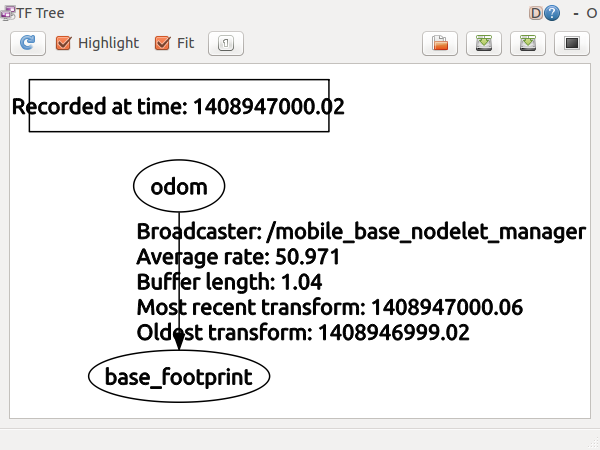
\includegraphics[width=0.8\columnwidth]{pictures/chapter10/rqt_tf_tree_kobuki.png}
\caption{tf\_tree를 통한 변환 확인}
\end{figure}

정말 장황한 토픽 설명을 마쳤다. ROS에서 각각의 프로세서인 노드간의 통신으로 토픽과 서비스, 액션 등을 이용하게 되는데 토픽은 그 중 가장 널리 사용되는 메시지 통신 방식으로 꼭 알아둬야 하는 부분이기 때문이다. 토픽에 대한 더 자세한 사항은 "ROS 정보 명령어 (rostopic)" 강좌를 참고하기 바라며 다음 강좌로 넘어가기로 하겠다.

%-------------------------------------------------------------------------------
\section{Kobuki 진단툴, 계기판, CUI 및 GUI 기능 테스트}\index{Kobuki 진단툴, 계기판, CUI 및 GUI 기능 테스트}

%-------------------------------------------------------------------------------
\subsection{진단 정보 (diagnostics information)}

로봇의 전원, 모터, 센서 그리고 내부 처리등의 에러 및 경고 메시지는 로봇 개발에서 필수적인 요소이다. 거북이 또한 이들의 정보를 제공하기 위하여  rqt\_robot\_monitor 를 통하여 이를 확인 할 수 있도록 돕고 있다. 사용방법은 GUI 를 사용하기에 매우 편리하다. 우선, 이를 위하여 아래의 명령어로 rqt\_robot\_monitor 를 설치하도록 하자.

\vspace{\baselineskip}
\begin{lstlisting}[language=ROS]
sudo apt-get install ros-indigo-rqt-robot-monitor
\end{lstlisting}


그 다음, 아래의 명령어로 rqt\_robot\_monitor 를 실행시키자.

\vspace{\baselineskip}
\begin{lstlisting}[language=ROS]
rosrun rqt_robot_monitor rqt_robot_monitor
\end{lstlisting}


아래의 그림과 같이, 로봇과 랩톱의 링크 와치독 정보, 배터리 상태, 범퍼, 절벽감지, 휠 드랍, 모터 전류, 자이로 센서값, 아날로그 디지털 입력값을 확인 가능하다. 아무런 문제가 없는 경우, 아래와 같이 표시된다.

\begin{figure}[h]
\centering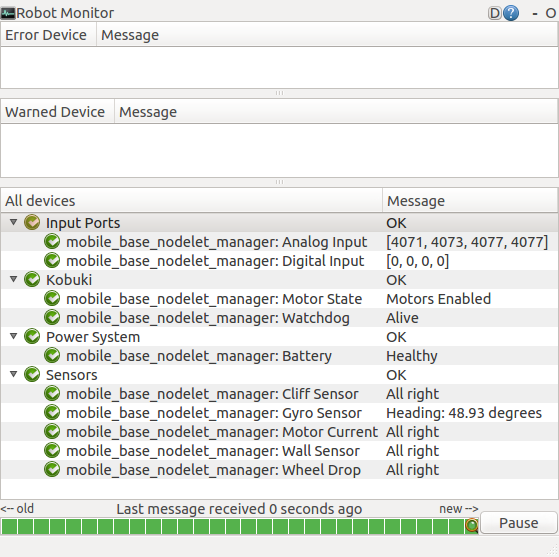
\includegraphics[width=0.8\columnwidth]{pictures/chapter10/rqt_robot_monitor.png}
\caption{rqt\_robot\_monitor를 통한 로봇 상태 파악}
\end{figure}

만약에, 문제가 있다면 아래와 같이 표시가 되는데 임의로 범퍼를 벽에 부딛쳤을때의 값이다. Warned Device 에 경고마크가 표시되며 문제를 알려준다.

\begin{figure}[h]
\centering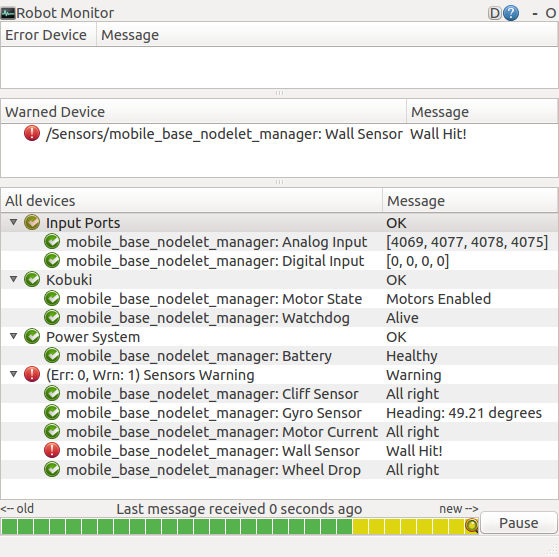
\includegraphics[width=0.8\columnwidth]{pictures/chapter10/diagnostics_warning.png}
\caption{진단 정보 (diagnostics information)}
\end{figure}

%-------------------------------------------------------------------------------
\subsection{계기판 (dashboard)}

거북이의 GUI 형태의 대쉬보드, 우리말로는 계기판을 소개한다. 이는 GUI 형태로 위에서 소개한 진단 정보를 포함하고 있고, 그 이외에도 각 종 메시지를 확인 가능한 콘솔(console), 모터 상태 파악, LED1, 2 제어, 거북이와 랩톱의 배터리 정보 확인들을 할 수 있다. 우선 관련 패키지를 설치하도록 하자.

\vspace{\baselineskip}
\begin{lstlisting}[language=ROS]
sudo apt-get install ros-indigo-kobuki-desktop
\end{lstlisting}

그 다음, 아래의 명령어로 kobuki\_dashboard 를 실행시키자.

\vspace{\baselineskip}
\begin{lstlisting}[language=ROS]
rosrun kobuki_dashboard kobuki_dashboard
\end{lstlisting}

아래의 그림과 같이, 정보를 확인하거나 LED를 제어 가능한 GUI 형태의 계기판을 실행되었다. 

각 부분을 클릭하면 아래와 같이 계기판이 추가된다. 하나 하나 테스트 해보기 바란다. 단, 필자가 이글을 작성하는 시점에서는 모터, 배터리에 대한 GUI가 이상하다. 나중에 관련 이슈를 보고해야 할 듯 싶다.

\begin{figure}[h]
\centering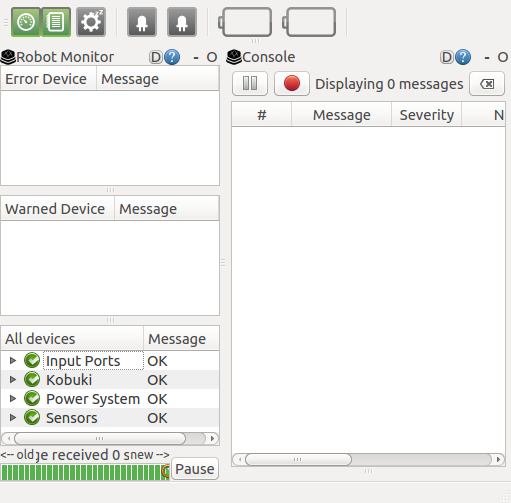
\includegraphics[width=0.7\columnwidth]{pictures/chapter10/kobuki_dashboard.png}
\caption{계기판 (dashboard)}
\end{figure}

%-------------------------------------------------------------------------------
\subsection{기능 테스트 (CUI 버전)}

거북이의 kobuki\_testsuite 패키지를 이용하면 거북이의 하드웨어를 테스트해 볼 수 있다. 각부분의 고장 여부를 파악하기에 좋은 패키지이다. 아래와 같이 kobuki\_testsuite 패키지의 다양한 노드를 실행 할 수 있다. 

\vspace{\baselineskip}
\begin{lstlisting}[language=ROS]
rosrun kobuki_testsuite %*노드명*)
\end{lstlisting}

사용 가능한 노드는 아래와 같다. 무한 회전, 이벤트 테스트, 자이로 테스트, 사운드 테스트 등이 있다. 어디까지나 하드웨어 테스트를 위한 노드들이기에 참고정도로만 해주자. 혹은, 각 파트가 파이썬으로 구성되어 있어서 관련 기능을 사용할 때 참고 소스로의 역할도 된다.

\vspace{\baselineskip}
\begin{lstlisting}[language=ROS]
inf_rotation.py
test_events.py
test_rotation.py
scan_angle.py
test_external_power.py
test_safewandering.py
test_analog_input.py
test_gyro.py
test_sounds.py
test_battery
test_input.py
test_translation.py
test_battery_voltage.py
test_led_array.py
test_digital_output.py
test_output.py 
\end{lstlisting}


실행 가능한 테스트중 에 "test\_events.py" 를 실행한 모습이 아래와 같다. 이벤트 발생을 위하여 처음에는 오른쪽 범퍼를 눌렀다가 띄었고, 로봇을 올려 들었다가 내려 놓았다. 관련된 범퍼, 휠 드랍, 절벽 감지 센서가 반응하여 이벤트가 발생되는 것을 확인 할 수 있다. 다른 테스트들은 각자 직접 해보기로 하자.

\vspace{\baselineskip}
\begin{lstlisting}[language=ROS]
$ rosrun kobuki_testsuite test_events.py
Try kobuki's hardware components; the following events should be reported:
  - buttons
  - bumpers
  - wheel drops
  - cliffs
  - plug/unplug adapter
  - dock/undock on base
  - charge completed
  - battery low/critical
  - digital input changes
[INFO] [WallTime: 1408952137.104793] Right bumper is pressed.
[INFO] [WallTime: 1408952137.185717] Right bumper is released.
[INFO] [WallTime: 1408952140.866974] Left wheel is dropped.
[INFO] [WallTime: 1408952140.886718] Right wheel is dropped.
[INFO] [WallTime: 1408952141.127440] Right side of robot is on the cliff.
[INFO] [WallTime: 1408952141.207462] Left side of robot is on the cliff.
[INFO] [WallTime: 1408952141.210328] Centre side of robot is on the cliff.
[INFO] [WallTime: 1408952141.627020] Left side of robot is on the floor.
[INFO] [WallTime: 1408952141.668215] Centre side of robot is on the floor.
[INFO] [WallTime: 1408952141.726817] Right side of robot is on the floor.
[INFO] [WallTime: 1408952141.807727] Left wheel is raised.
[INFO] [WallTime: 1408952141.847553] Right wheel is raised.
\end{lstlisting}

%-------------------------------------------------------------------------------
\subsection{기능 테스트 (GUI 버전)}

좀 전에 설명한 "kobuki\_testsuite" 패키지가 CUI (Character User Interface) 기반 이였다면 이번에 소개할 kobuki\_qtestsuite 는 GUI (Graphical user interface) 기반이다. 사용방법은 아래와 같다. 단, 일반 사용자를 위한 패키지이기보다는 출하전 테스트, 로봇 및 배터리 생명 주기 등을 테스트하는 프로그램이 아닐까하는 생각이 든다.

\vspace{\baselineskip}
\begin{lstlisting}[language=ROS]
$ sudo apt-get install ros-indigo-kobuki-qtestsuite
. /opt/ros/indigo/setup.bash
kobuki_qtestsuite
\end{lstlisting}

\begin{figure}[h]
\centering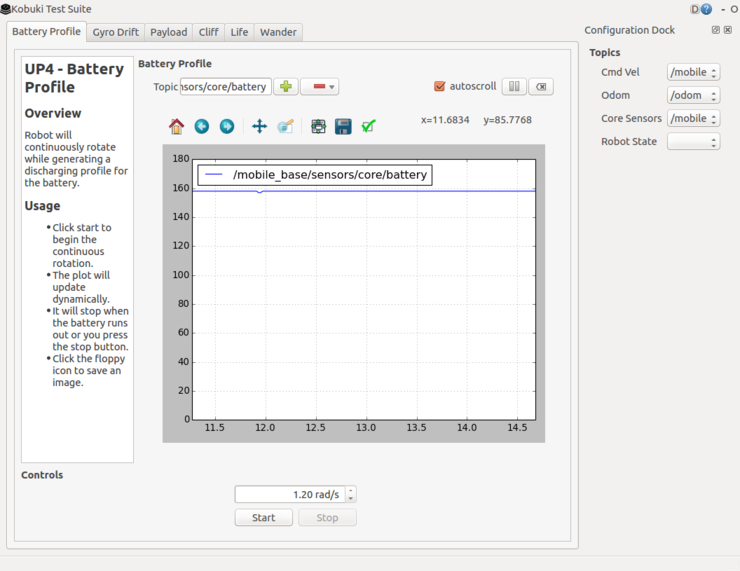
\includegraphics[width=0.9\columnwidth]{pictures/chapter10/kobuki_qtestsuite.png}
\caption{kobuki\_qtestsuite를 이용한 기능 테스트}
\end{figure}

Kobuki의 진단툴, 계기판, CUI 및 GUI 기능 테스트 관련 패키지에 대해서 알아 보았다. 본질에서 벗어나는 부가적인 강좌가 되어 버렸지만 앞서 말한바와 같이 kobuki\_testsuite의 각 기능들을 살펴보면 나중에 거북이 관련 프로그래밍에 큰 도움이 될 듯 싶다. 그러면 또 다음 강좌로 넘어가 보자.

%-------------------------------------------------------------------------------
\section{Kobuki 펌웨어 업그레이드}\index{Kobuki 펌웨어 업그레이드}

%-------------------------------------------------------------------------------
\subsection{펌웨어 버전 확인}

거북이의 펌웨어를 확인하기 위한 방법으로는 2가지가 존재한다. 하나의 "kobuki\_node"를 실행할 때, "--screen" 옵션을 붙여주는 방법과 또 다른 하나는 "kobuki\_node"를 실행 후에 "/mobile\_base/version\_info" 토픽을 살펴보는 방법이다.

%-------------------------------------------------------------------------------
\subsubsection{kobuki\_node 실행시에 펌웨어 버전 확인하기 }

아래의 명령어 처럼, "--screen" 옵션을 붙여주면 노드가 실행되면서 버전 정보를 확인할 수 있다. 필자의 경우, 구입한지 오래되어 버전이 한 단계 낮았었다.

\vspace{\baselineskip}
\begin{lstlisting}[language=ROS]
$ roslaunch kobuki_node minimal.launch --screen
[ INFO] [1408612929.814111512]: Kobuki : Version info - Hardware: 1.0.4. Firmware: 1.1.4
\end{lstlisting}


%-------------------------------------------------------------------------------
\subsubsection{kobuki\_node가 발행하는 토픽을 통해 펌웨어 버전 확인하기}

\vspace{\baselineskip}
\begin{lstlisting}[language=ROS]
$ rostopic echo /mobile_base/version_info 
hardware: 1.0.4
firmware: 1.1.4
software: 0.6.0
udid: [98107192, 825317169, 1460173122]
features: 3
---
\end{lstlisting}

%-------------------------------------------------------------------------------
\subsection{펌웨어 버전 업데이트 하기}

%-------------------------------------------------------------------------------
\subsubsection{관련 파일 및 프로그램 다운로드}

아래와 같이 거북이의 펌웨어\footnote{\url{http://kobuki.yujinrobot.com/home-en/documentation/howtos/upgrading-firmware/upgrading-firmware-linux/}} hex\footnote{\url{http://files.yujinrobot.com/kobuki/firmware/}} 파일 및 이를 거북이에 업로드 할 수 있도록하는 프로그램인 stm32flash\footnote{\url{http://stm32flash.googlecode.com/}}를 다운로드 하자. stm32flash 은 make 해두어 실행 가능한 상태로 만들어 둔다. 

\vspace{\baselineskip}
\begin{lstlisting}[language=ROS]
$ mkdir ~/firmware_update
cd ~/firmware_update
wget http://stm32flash.googlecode.com/files/stm32flash.tar.gz
wget http://files.yujinrobot.com/kobuki/firmware/kobuki_firmware-latest.hex
tar -xvf stm32flash.tar.gz
cd stm32flash
make
\end{lstlisting}


%-------------------------------------------------------------------------------
\subsubsection{펌웨어 다운로드}

우선, 로봇 전원을 끄자. 그 뒤 아래의 그림의 펌웨어 다운로드 기능으로 전환하는 스위치를 "Download" 쪽으로 스위칭한 후, 거북이 전원을 다시 킨다. 전원을 키는가 동시에 아래의 명령을 내려주면 펌웨어가 업로드되고 업데이트 된다. 여기서 옵션으로 "/dev/ttyUSB0" 으로 포트를 선언하였는데 이는 사용자마다 다를 듯 싶다. 주의하기 바란다.

\vspace{\baselineskip}
\begin{lstlisting}[language=ROS]
$ ./stm32flash -b 115200 -w ../kobuki_firmware-latest.hex /dev/ttyUSB0
\end{lstlisting}

\begin{figure}[h]
\centering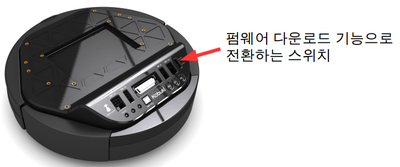
\includegraphics[width=0.4\columnwidth]{pictures/chapter10/firmware_download.png}
\caption{펌웨어 다운로드 모드 변환 스위치}
\end{figure}

업데이트를 마쳤으면, 스위치를 원래 상태로 돌리고 로봇을 재부팅하면 완료된다. 제대로 되었는지 확인하기 위해서 앞에서 설명한 방법 중 하나를 실행하면 된다. 아래와 같이 펌웨어가 최신 버전으로 업데이트 되었음을 확인할 수 있다.

\vspace{\baselineskip}
\begin{lstlisting}[language=ROS]
$ roslaunch kobuki_node minimal.launch --screen
[ INFO] [1408953316.298156409]: Kobuki : Version info - Hardware: 1.0.4. Firmware: 1.2.0
\end{lstlisting}

%-------------------------------------------------------------------------------
\section{Kobuki 자동 도킹}\index{Kobuki 자동도킹}

%-------------------------------------------------------------------------------
\subsection{거북이와 도킹 스테이션}

거북이는 자동 충전을 위하여 아래의 오른쪽 사진과 같은 도킹 스테이션이라는 별도의 충전소를 가지고 있다. 이 도킹 스테이션은 내부적으로는 충전 어댑터를 내부에 포함하고 있어서 외부에 돌출된 충전단자를 통해 로봇과 연결되어 로봇에 탑재된 배터리를 충전하게 된다.

이 때에 사용되는 하드웨어적인 구성으로는 도킹 스테이션에 적외선(IR) 발신부 3개 (중앙, 좌/우측)와 거북이 본체에 적외선 수신부 3개, 그리고 도킹을 위한 도킹 단자와 충전 상태 표시 LED 로 구성되어 있다.

참고로, 도킹을 위해서는 도킹 스테이션과 로봇은 도킹 스테이션을 기준으로 수평 2미터, 수직 정면 방향으로 5미터 정도의 구간에서 정확한 동작을 하게 되어 있다. 또한 도킹 스테이션의 앞에는 아무런 장애물이 없어야 한다.

\begin{figure}[h]
\centering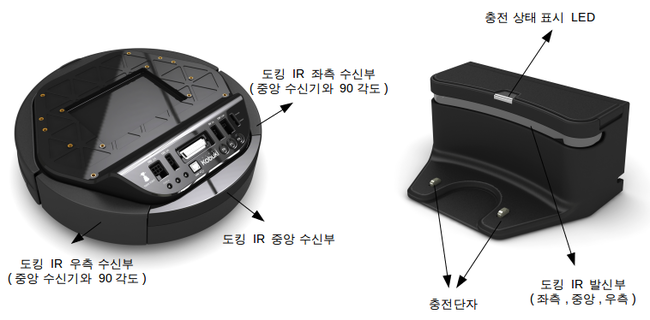
\includegraphics[width=0.8\columnwidth]{pictures/chapter10/kobuki_docking_station.png}
\caption{거북이와 도킹 스테이션}
\end{figure}

\begin{figure}[h]
\centering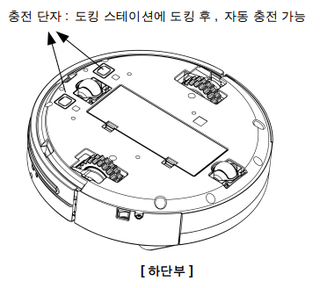
\includegraphics[width=0.5\columnwidth]{pictures/chapter10/recharge.png}
\caption{도킹후 충전에 사용되는 충전 단자}
\end{figure}

%-------------------------------------------------------------------------------
\subsection{도킹과 자동 충전}

도킹을 위한 패키지로는 kobuki\_auto\_docking\footnote{\url{http://wiki.ros.org/kobuki_auto_docking}} 가 제공된다. 이를 실행하기 위한 방법은 아래의 2가지가 존재한다. 사용하기 편한 실행 방법을 하나만 선택하여 실행시켜 주도록 하자.

%-------------------------------------------------------------------------------
\subsubsection{추가 노드 실행}

\vspace{\baselineskip}
\begin{lstlisting}[language=ROS]
$ roslaunch kobuki_node minimal.launch --screen 
\end{lstlisting}

위와 같이 minimal.launch 가 실행되어 있다면 아래와 같이 도킹 관련만 추가로 실행시켜주면 된다.
 
\vspace{\baselineskip}
\begin{lstlisting}[language=ROS]
$ roslaunch kobuki_auto_docking minimal.launch --screen
\end{lstlisting} 

%-------------------------------------------------------------------------------
\subsubsection{도킹 포함 런치 실행}

만약에 위의 두 가지 모두를 한꺼번에 실행하고자 할 경우에는 아래와 같은 런치 파일을 실행해 주면 된다.

\vspace{\baselineskip}
\begin{lstlisting}[language=ROS]
$ roslaunch kobuki_auto_docking compact.launch --screen
\end{lstlisting} 

%-------------------------------------------------------------------------------
\subsubsection{도킹 실행}

원래, 배터리가 일정 수준 이하일때 아래와 같이 도킹을 수행하도록 프로그래밍하면 되지만 여기서는 테스트를 위하여 임의로 도킹 노드를 활성화 하도록 하겠다. 아래의 명령어로 도킹을 수행하자. 도킹 명령을 주게되면 아래의 동영상 처럼 거북이는 도킹 스테이션을 찾고, 도킹 스테이션의 수직 방향으로 접근 후, 도킹. 그리고 자동으로 충전 상태로 들어가게 된다.

\vspace{\baselineskip}
\begin{lstlisting}[language=ROS]
$ roslaunch kobuki_auto_docking activate.launch --screen
\end{lstlisting}

\begin{figure}[h]
\centering
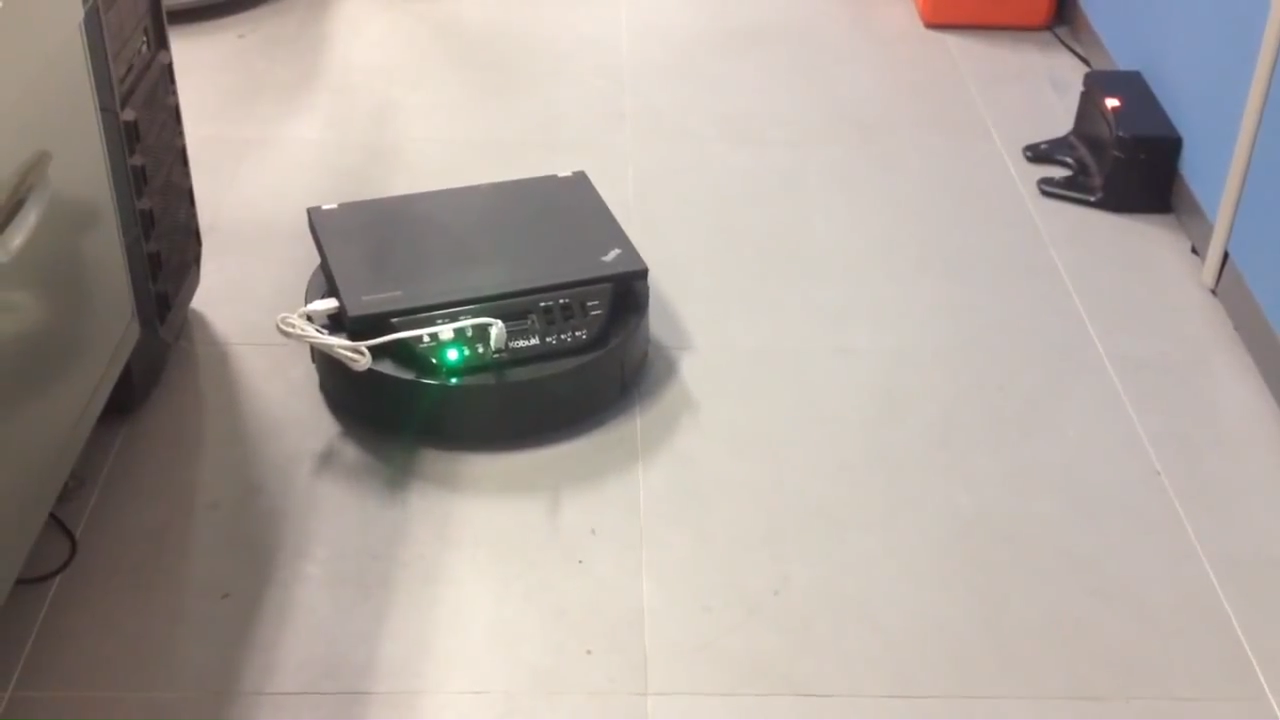
\includegraphics[width=0.4\columnwidth]{pictures/chapter10/kobuki_docking1.png}
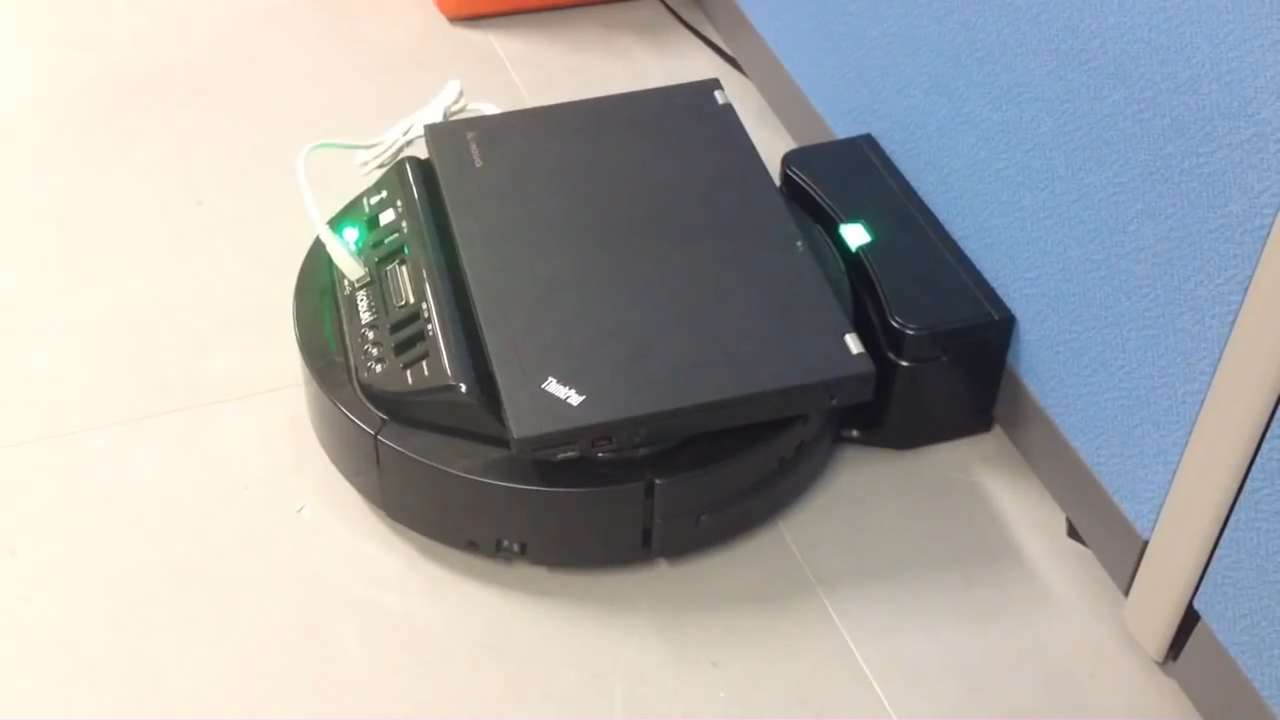
\includegraphics[width=0.4\columnwidth]{pictures/chapter10/kobuki_docking2.png}
\caption{도킹과 자동 충전}
\end{figure}


\vspace{\baselineskip}
\textbf{[참고사항]} 거북이의 상태 표기 LED : 상태 표기 LED (Status LED)는 패널의 맨 왼쪽에 위치하고 있으며, 거북이의 현재 배터리 상태를 표기함
\begin{itemize}[leftmargin=*]
\item {\color{limegreen}녹색}: 기본 상태로 배터리가 충전되어 있음을 나타냄
\item \textcolor{orange}{주황색}: 배터리의 잔량이 낮은 상태를 나타냄 (충전이 필요한 상태임)
\item {\color{limegreen}녹색 점멸}: 배터리가 충전 중임을 나타냄
\end{itemize}

\vspace{\baselineskip}
\textbf{[참고사항]} 도킹스테션의 상태 표기 LED : 충전 상태 표기 LED는 현재 충전 상태를 표기함
\begin{itemize}[leftmargin=*]
\item \textcolor{red}{적색}: 로봇이 도킹되어 있지 않은 상태
\item {\color{limegreen}녹색 점멸}:: 로봇이 도킹되어 충전 중인 상태
\item {\color{limegreen}녹색}: 로봇이 도킹되어 있고, 충전이 완료된 상태
\end{itemize}

%-------------------------------------------------------------------------------
\subsection{도킹 알고리즘}

도킹 적외선 발신부, 수신부가 어느 정도의 파워로 범위로 작동되는지 알 수 없는 상황에서 도킹 알고리즘을 정확히 분석하는 것은 어려워 보인다. 다만, 거북이는 참고자료\footnote{\url{http://wiki.ros.org/kobuki/Tutorials/Testing\%20Automatic\%20Docking}}에서 이와 관련된 알고리즘을 위키에 설명하고 있고, 관련 소스\footnote{\url{https://github.com/yujinrobot/kobuki/blob/indigo/kobuki_auto_docking/src/auto_docking_ros.cpp}}에서 공개하고 있다. 아래의 알고리즘은 그 참고 자료들을 바탕으로 설명하였다.

우선, 도킹 스테이션의 적외선 발신부는 총 3군데로 아래의 그림과 같이 중앙과 좌측, 우측에 위치해 있다. 이 3개의 적외선 발신부로 도킹 스테이션 앞에는 중앙영역, 좌측영역, 우측영역이 만들어지고, 거리에 따라 가까운 거리, 먼 거리 두 가지로 나뉜다. 이것으로 아래와 같이 총 7가지 패턴이 만들어 진다. 

\vspace{\baselineskip}
\begin{lstlisting}[language=ROS]
NONE  =  0
NEAR_LEFT =  1
NEAR_CENTER =  2
NEAR_RIGHT =  4
FAR_LEFT = 16
FAR_CENTER  =  8
FAR_RIGHT = 32
\end{lstlisting}

\begin{figure}[h]
\centering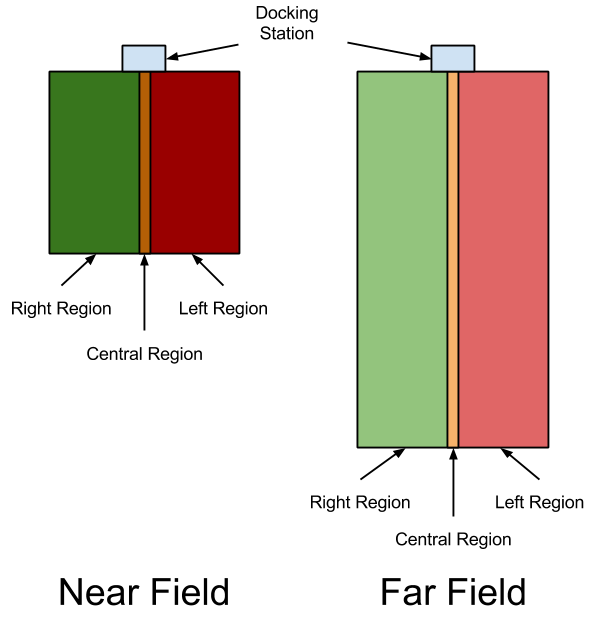
\includegraphics[width=0.8\columnwidth]{pictures/chapter10/docking_region.png}
\caption{도킹 스테이션의 적외선 발신 범위}
\end{figure}

(출처:참고자료[2])


거북이 본체에는 도킹 스테이션에서 발신한 적외선을 수신 할 수 있는 수신부가 아래와 같이 3개를 보유하고 있다. 만약 거북이가 도킹 스테이션에서 발신한 적외선을 수신할 수 있는 영역에 있다면, kobuki\_auto\_docking 노드가 실행 가능하다. 그 영역은 앞서 말한바와 같이 도킹 스테이션을 기준으로 수평 2미터, 수직 정면 방향으로 5미터 정도이다. 로봇은 도킹을 위해 제자리에서 회전하며, 3곳의 적외선 수신부 중 한 곳 이상에서 적외선이 감지되면 도킹 작업을 수행하게 된다. 

아래의 명령어로 도킹과 관련한 센서 정보를 토픽을 통해 확인 할 수 있다.

\vspace{\baselineskip}
\begin{lstlisting}[language=ROS]
$ rostopic echo /mobile_base/sensors/dock_ir
---
header: 
  seq: 17202
  stamp: 
    secs: 1408965261
    nsecs: 393052992
  frame_id: dock_ir_link
data: [0, 0, 32]
---
\end{lstlisting}


현재, 오른쪽에 위치한 적외선 수신부(data[2])가 32이므로 이는 거북이가 도킹 스테이션의 우측 영역에서 멀리 떨어져 있다는 것을 의미한다.

\begin{figure}[h]
\centering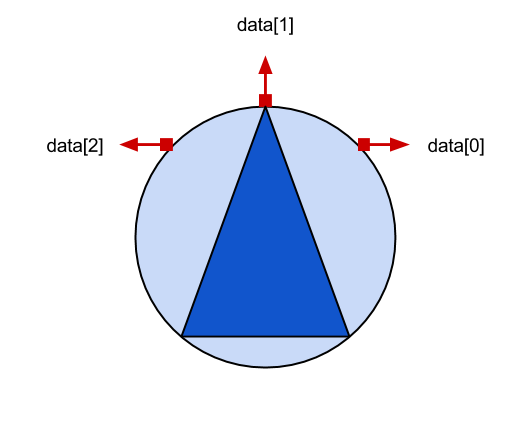
\includegraphics[width=0.7\columnwidth]{pictures/chapter10/dock_ir.png}
\caption{적외선 수신부의 위치와 방향}
\end{figure}

(출처:참고자료[2])

이와 같이 거북이는 도킹 스테이션의 적외선 발신부와 거북이 본체의 적외선 수신부를 이용하여 도킹을 수행하게 되는데 그 흐름 예를들어 설명하면 아래와 같은 3가지 패턴이라고 볼 수 있다.


\setcounter{num}{0}

\vspace{\baselineskip}
\noindent
\stepcounter{num}
\thenum) 로봇이 도킹 스테이션의 중앙 지역에 위치한 경우
:  도킹 충전단자에 닫기 전까지 바로 직진하여 도킹하게 된다.

\vspace{\baselineskip}
\noindent
\stepcounter{num}
\thenum) 로봇이 좌측 영역에 위치한 경우
: 우측 적외선 수신부(data[0])에 도킹 스테이션의 좌측 영역의 신호를 감지할 때 까지 반시계 방향으로 돌게 된다. 좌측 영역의 신호를 감지하면 로봇은 직진하게 되고 중앙 지역까지 가게 된다. 여기서도 마찬가지로 반시계 반향으로 회전하게 되고, 중앙 적외선 수신부(data[1])이 도킹 스테이션의 중앙 영역의 신호를 감지하게 되면 직진하여 도킹하게 된다.

\vspace{\baselineskip}
\noindent
\stepcounter{num}
\thenum) 로봇이 우측 영역에 위치한 경우
: 방향만 다를뿐 2번과 같은 알고리즘으로 동작하게 된다.

현재, 도킹 알고리즘은 측정  지역을 벗어난 경우 및 반응 속도면에서 개선점이 보인다. 관심있는 분은 새로운 도킹 알고리즘을 제안해 보는것도 좋을 듯 싶다.


%-------------------------------------------------------------------------------
\section{Kobuki 시뮬레이션 (RViz)}\index{Kobuki 시뮬레이션 (RViz)}

%-------------------------------------------------------------------------------
\subsection{가상 시뮬레이션}

거북이는 로봇 본체 없이 가상 로봇을 이용하여 프로그램밍하고 가상 시뮬레이션을 통해 개발하는 것을 지원하고 있다. 그 방법으로는 2가지가 있는데, 하나는 ROS의 3차원 시각화 툴인 RViz 를 이용하는 것이고, 또 다른 하나는 3차원 로봇 시뮬레이터 Gazebo를 이용하는 것이다. 이번 강좌에서는 그 중 첫 번째인 RViz를 이용하는 방법에 대해 알아 보도록 하겠다. 거북이 본체없이 거북이의 구동, 네비게이션을 시험해보기 원하는 유저에게는 강력 추천한다. 로봇 본체 없이도 시뮬레이션을 할 수 있도록 kobuki\_soft\footnote{\url{http://wiki.ros.org/kobuki_soft}} 를 공개해준 개발자 Jihoon Lee 님에게 이 자리를 빌어 감사하다는 말을 전하고 싶다.

%-------------------------------------------------------------------------------
\subsection{kobuki\_soft 메타 패키지}

kobuki\_soft 는 많이 알려지지는 않았지만 ROS의 시각화툴인 RViz 환경에서 거북이의 동작을 시뮬레이션 할 수 있는 가상 시뮬레이션 환경을 제공해주는 메타 패키지이다. 포함된 패키지로는 가상 거북이 구동과 관련된 kobuki\_softnode 와 네비게이션 정보를 담고 있는 kobuki\_softapps 가 있다. 

\vspace{\baselineskip}
\begin{description}
\item[kobuki\_soft (메타 패키지)]
\item[위키]: \url{http://wiki.ros.org/kobuki_soft}
\item[저장소]: \url{https://github.com/yujinrobot/kobuki_soft}
\end{description}

\setcounter{num}{0}

\vspace{\baselineskip}
\noindent\stepcounter{num}
\thenum) \textbf{kobuki\_softnode}
\begin{description}
\item[위키]: \url{http://wiki.ros.org/kobuki_softnode}
\item[기능]: 거북이 시뮬레이션과 관련된 가상 로봇 시뮬레이션 기능의 패키지이다. RViz 에서 실행 가능하다.
\end{description}

\vspace{\baselineskip}
\noindent\stepcounter{num}
\thenum) \textbf{kobuki\_softapps}
\begin{description}
\item[위키]: \url{http://wiki.ros.org/kobuki_softapps}
\item[기능]: kobuki\_softnode 와 연관되는 패키지로 시뮬레이션 관련 애플리케이션을 가지고 있으며 주로 네비게이션을 다루고 있다.
\end{description}

가상시뮬레이션을 이용하기 위해서는 kobuki\_soft 패키지를 아래와 같이 설치하면 된다.

\vspace{\baselineskip}
\begin{lstlisting}[language=ROS]
$ sudo apt-get install ros-indigo-kobuki-soft
\end{lstlisting}

%-------------------------------------------------------------------------------
\subsection{가상 로봇 실행}

우선, 아래와 같이 거북이 소프트노드를 구동한다. 이 런치 파일을 실행하게 되면 kobuki\_description 패키지에서 거북이의 3차원 모델을 불러오고, 거북이 노드와 동일한 mobile base nodelet manager, mobile base, diagnostic aggregator, robot state publisher 노드들을 가상으로 동작하게 끔 만들어둔 kobuki\_softnode를 실행하게 된다.

이는 내부적으로 turtle\_teleop\_key 노드에서 발행하는 velocity, motor\_power 등의 구동 명령어를 받아서 가상의 구동을 하게 된다. 예를 들어, 속도 명령을 받아서 오드메트리(odometry) 정보를 만들어 토픽으로 발행하게 된다. 마찬가지로 joint states 및 tf 도 발행하게 하여 RViz 에서 거북이의 움직임을 확인할 수 있도록 해준다.

단, 센서 정보는 RViz 에서 사용할 수 없기 때문에 이를 위해서는 물리엔진이 포함된 3차원 시뮬레이터 Gazebo 를 이용해야 한다.  이 부분에서 대해서는 다음 강좌에서 설명하기로 하고 이번 강좌에서는 간단한 이동과 주어진 지도상에서 네비게이션하는 내용만 담도록 하겠다.
 
\vspace{\baselineskip}
\begin{lstlisting}[language=ROS]
$ roslaunch kobuki_softnode full.launch
\end{lstlisting}

그 다음, RViz 를 실행하고, 추가로 왼쪽 디스플레이창(Displays) 의 Global Options 의 fixed frame을 "/odom" 으로 바꿔준다. 그리고 난 후, 디스플레이창의 왼쪽 하단 부분의 "Add" 버튼을 눌러, 디스플레이 중 "RobotModel" 을 클릭하여 추가하도록 하자. 이미 full.launch 런치 파일에서 거북이 3차원 모델을 불러온 상태이기 때문에 아래의 그림과 이 거북이의 3차원 모델이 중앙에 표시 될 것이다.

\vspace{\baselineskip}
\begin{lstlisting}[language=ROS]
$ rosrun rviz rviz
\end{lstlisting}

\begin{figure}[h]
\centering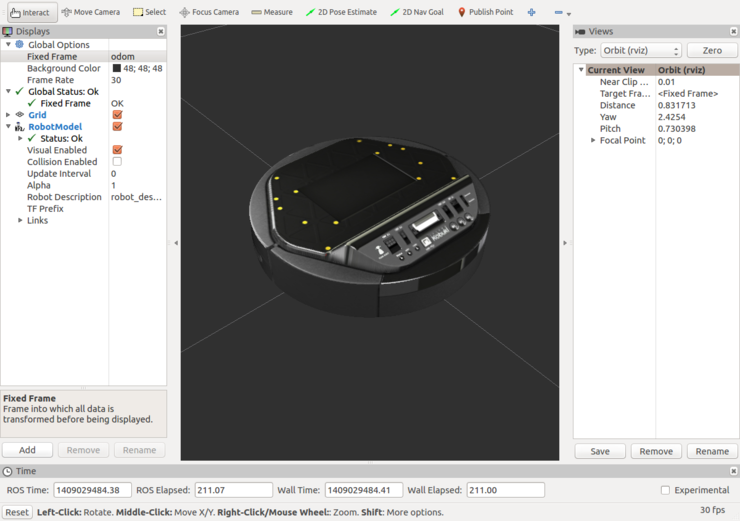
\includegraphics[width=0.9\columnwidth]{pictures/chapter10/rviz_kobuki.png}
\caption{가상 로봇 실행}
\end{figure}

자! 그럼 다음에는 가상의 로봇을 구동시켜 보자. 지금까지 사용하였던 keyop.launch 런치파일을 실행하여 키보드로 직접 구동시켜 보자. 

\vspace{\baselineskip}
\begin{lstlisting}[language=ROS]
$ roslaunch kobuki_keyop keyop.launch
\end{lstlisting}

\begin{itemize}[leftmargin=*]
\item 방향키 ↑ : 리니어 속도 지정으로 전진 방향으로 이동한다. (0.5씩, 단위 = m/sec) 
\item 방향키 ↓ : 리니어 속도 지정으로 후진 방향으로 이동한다. (0.5씩, 단위 = m/sec) 
\item 방향키 ← : 회전 속도 지정으로 시계 반대 방향으로 회전한다. (0.33씩, 단위 = rad/sec) 
\item 방향키 → : 회전 속도 지정으로 시계 방향으로 회전한다. (0.33씩, 단위 = rad/sec) 
\item 스페이스바 : 리니어 속도 및 회전 속도를 초기화 한다.
\item d : 모터를 비활성화 한다. (구동 불가능 상태)
\item e : 모터를 활성화 한다. (구동 가능 상태)
\item q : 종료
\end{itemize}

%-------------------------------------------------------------------------------
\subsection{odom 토픽 확인}

구동을 확인했으니 오도메트리(odometry) 정보가 제대로 생성되고 발행되는지 확인해보자. 아래와 같이 rostopic 명령어로 확인할 수 도 있을 것이지만, 이번에는 RViz 를 하고 있기때문에 시각적으로 확인해보자. RViz 의 왼쪽 하단의 "Add"를 클릭 후, 나오는 시각화 생성 화면에서 "By Topic" 탭을 클릭하고, "Odometry" 를 선택하여 추가하도록 하자. 그러면 화면의 거북이의 전진방향으로 오도메트리를 나타내는 빨간색 화살표가 나타난다. 화살표 초기 값이 매우 크기 때문에 왼쪽 디스플레이창의 "Odometry"의 세부 옵션인 "Length" 의 값을 0.5로 설정하도록 하자.

\vspace{\baselineskip}
\begin{lstlisting}[language=ROS]
$ rostopic echo /odom
\end{lstlisting}

\begin{figure}[h]
\centering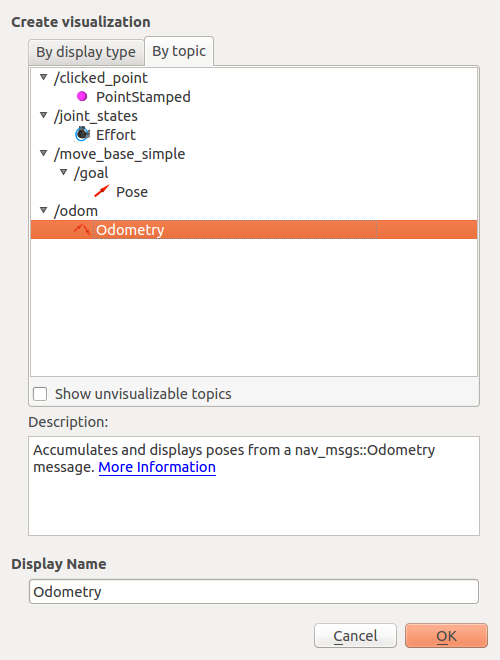
\includegraphics[width=0.5\columnwidth]{pictures/chapter10/rviz_odom.png}
\caption{odom 토픽 확인을 위한 odometry 디스플레이 추가}
\end{figure}

이제 다시 "keyop.launch" 노드를 이용하여 가상의 거북이를 움직여보자. 좀 전과는 달리 빨간 화살표가 로봇의 궤적에 따라 표시됨을 확인할 수 있을 것이다. 이 오도메트리 정보는 이동 로봇에 있어서는 자기 자신이 어디에 있는지에 대한 정보의 기본이 되기 때문에 매우 기본적인 요소이다. 일단, 오도메트리 정보가 제대로 표시되는지만 체크하였다.

\begin{figure}[h]
\centering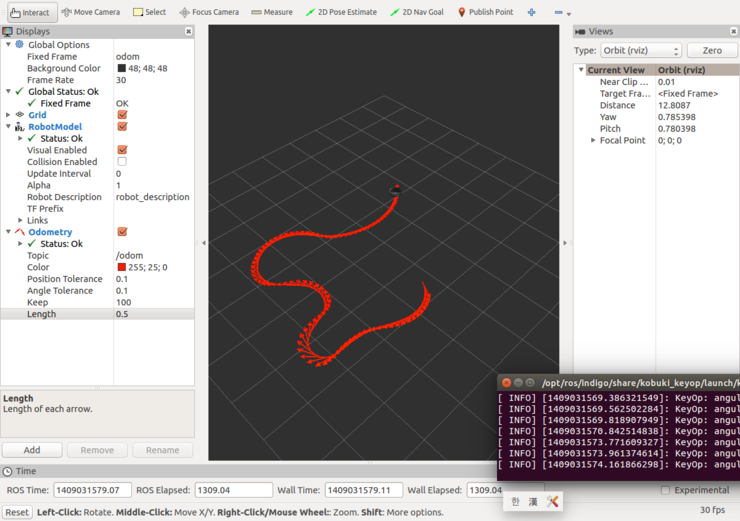
\includegraphics[width=0.9\columnwidth]{pictures/chapter10/rviz_kobuki_keyop_launch.png}
\caption{keyop.launch를 이용한 가상 로봇 이동}
\end{figure}

%-------------------------------------------------------------------------------
\subsection{tf 토픽 확인}

거북이 구성 요소들의 상대 좌표 정보를 담은 tf의 경우 이전처럼 rostopic 명령어로 확인할 수 있지만 odom 과 마찬가지로 RViz 로 확인해보고, 계층 구조에 대해서는 rqt\_tf\_tree 를 통하여 살펴보도록 하자. 이번에는 RViz 의 왼쪽 하단의 "Add"를 클릭 후, 나오는 시각화 생성 화면에서 "TF" 를 선택하여 추가하도록 하자. 그러면 화면의 거북이 모델에 odom, base\_footprint, gyro\_link, wheel\_left\_link, wheel\_right\_link 등이 표시된다. 여기서, 다시 "keyop.launch" 노드를 이용하여 가상의 거북이를 움직여보자. 거북이가 움직이면서 wheel\_left\_link, wheel\_right\_link 의 tf 마크가 회전하는 것을 아래의 동영상처럼 확인할 수 있을 것이다.

\begin{figure}[h]
\centering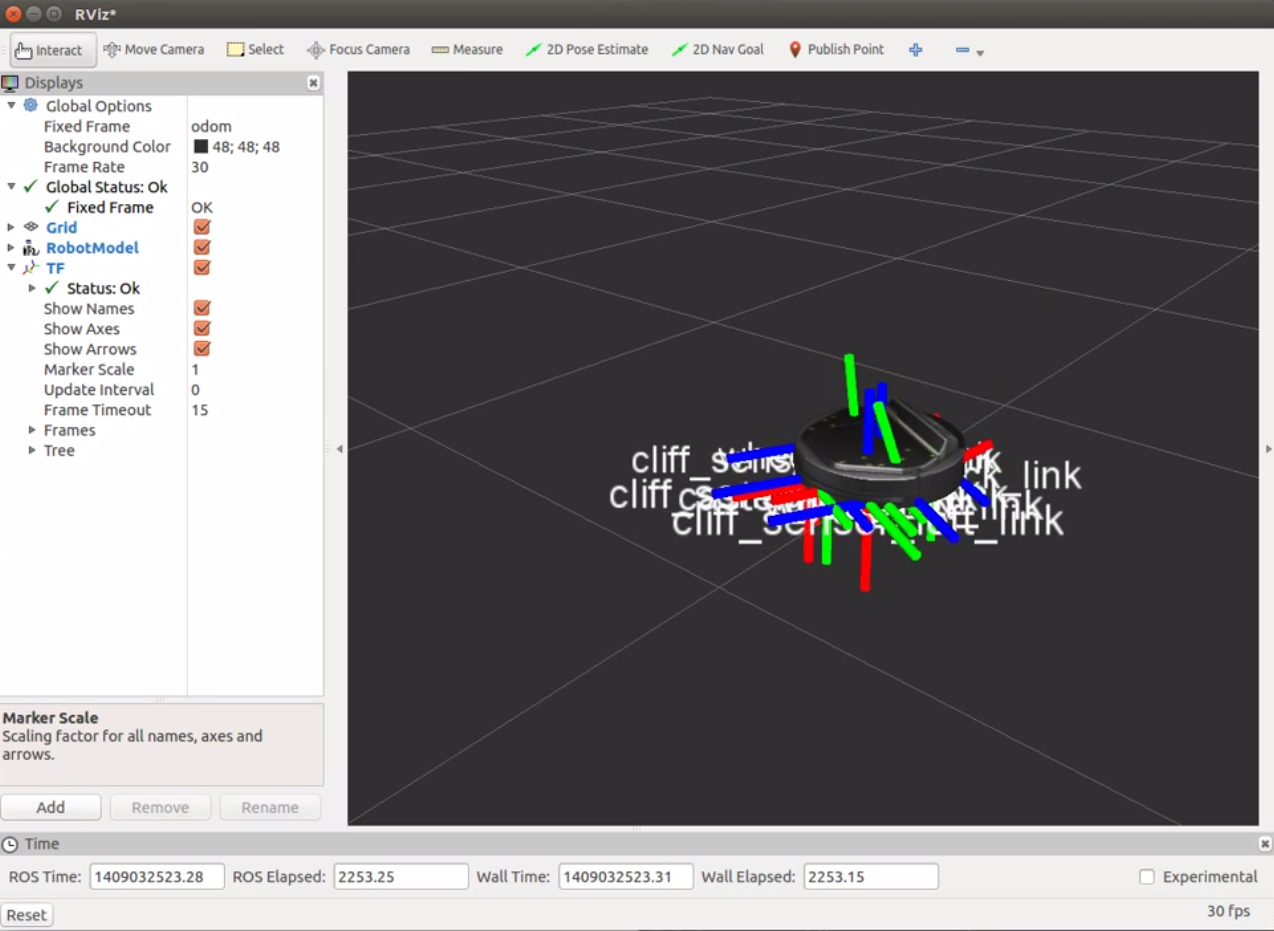
\includegraphics[width=0.9\columnwidth]{pictures/chapter8/rviz_kobuki_tf.png}
\caption{RViz에서의 tf 토픽 확인}
\end{figure}

이번에는 아래 명령어로 rqt\_tf\_tree 를 실행하도록 하자. 그러면 아래의 그림과 같이, 각 부분의 요소들이 tf 로 상대 위치가 변환되어 연관되어 있음을 확인할 수 있다. 이를 통해 나중에는 로봇위에 장착하는 센서들의 위치등도 표현 가능하다. 이 부분에 대한 자세한 사항은 네비게이션 강좌로 넘기기로 하겠다.

\vspace{\baselineskip}
\begin{lstlisting}[language=ROS]
$ rosrun rqt_tf_tree rqt_tf_tree 
\end{lstlisting}

\begin{figure}[h]
\centering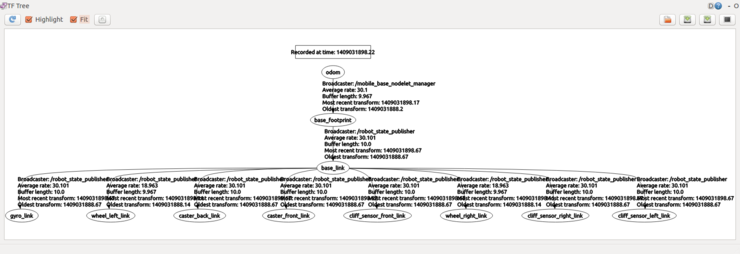
\includegraphics[width=0.9\columnwidth]{pictures/chapter10/rqt_tf_tree_kobuki_tf.png}
\caption{rqt\_tf\_tree를 통한 tf 토픽 확인}
\end{figure}

%-------------------------------------------------------------------------------
\subsection{가상 네비게이션}

kobuki\_soft 패키지에는 가상 네비게이션이 포함되어 있다. 이를 사용하기 위해서는 추가적으로 몇가지 패키지를 더 설치해 주도록 하자. 이번에 설치하는 패키지는 ROS 의 대표적인 패키지인 navigation 패키지와 유진로봇사의 맵이다. 설치 명령어는 아래와 같다.

\vspace{\baselineskip}
\begin{lstlisting}[language=ROS]
$ sudo apt-get install ros-indigo-navigation ros-indigo-yujin-maps
\end{lstlisting}

필수 패키지를 설치하였으면, 지금까지 실행된 모든 노드를 종료하고 아래와 같이 네비게이션 데모만 실행하도록 하자. 실행하면 아래의 첨부 그림과 같이 RViz 가 자동으로 구동되며 네비게이션에 필요한 모든 환경을 구축해 두었을 것이다. 여기서 네비게이션은 SLAM 으로 지도를 작성 후에  작성된 맵 위에서 지정된 위치로 로봇을 이동시키는 것을 의미한다. 이 부분에 자세한 내용은 차후에 네비게이션 강좌에서 더 자세히 다루기로 하겠다. 일단, RViz 의 중앙 상단의 "2D Nav Goal" 을 클릭하여 지도상의 임의의 위치에 클릭 하고 드래그하여 위치와 방향을 설정하자. 그러면 로봇은 장애물을 피하고 이동하게 된다. 

단, 개발자에게 문의한 결과, RViz 환경만을 쓴 시뮬레이션이라 로봇의 Odometry와 모터의 시뮬레이션만을 목적으로 하였고 외부 정보를 센싱할 수 없어서 벽등에 충돌한다고 밝혔다. 이를 위해서는 거북이의 또다른 시뮬레이션인 stage 및 gazebo 에서 다루어 지고 있다고 한다. 이에 대한 내용은 다음 강좌에 더 자세히 다루도록 하자.

\vspace{\baselineskip}
\begin{lstlisting}[language=ROS]
$ roslaunch kobuki_softapps nav_demo.launch
\end{lstlisting}

\begin{figure}[h]
\centering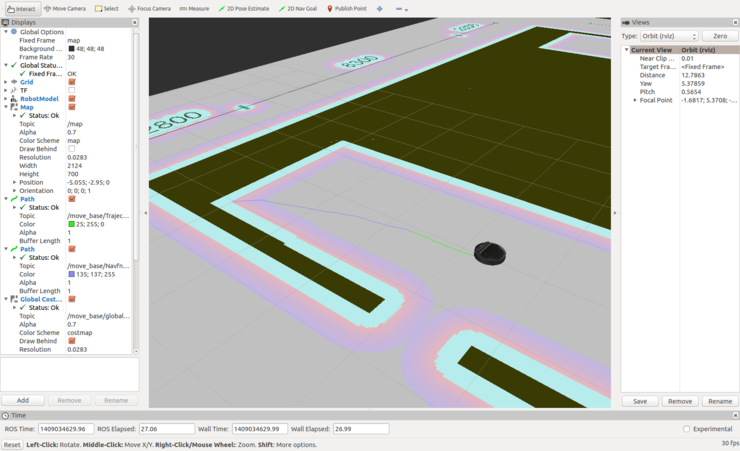
\includegraphics[width=0.5\columnwidth]{pictures/chapter10/nav_demo.png}
\caption{nav\_demo.launch를 실행한 모습}
\end{figure}

RViz 를 이용한 거북이의 가상 시뮬레이션에 대해서 간략히 알아보았다. 더 자세한 시뮬레이션에 대한 내용은 거북이의 네비게이션 강좌를 마치고 추가로 진행할 예정이다.

%-------------------------------------------------------------------------------
\section{Kobuki 시뮬레이션 (Gazebo)}\index{Kobuki 시뮬레이션 (Gazebo)}

%-------------------------------------------------------------------------------
\subsection{Gazebo}\index{gazebo}

\begin{figure}[h]
\centering
\includegraphics[width=0.3\columnwidth]{pictures/chapter10/gazebo.png}
\caption{gazebo}
\end{figure}

가제보(Gazebo\footnote{\url{http://gazebosim.org/}})는 로봇 개발에 필요한 3차원 시뮬레이션을 위한 로봇, 센서, 환경 모델 등을 지원하고 물리 엔진을 탑재하여 실제와 근사한 결과를 얻을 수 있는 3차원 시뮬레이터이다. 

로봇을 위한 2/3차원 시뮬레이터\footnote{\url{http://en.wikipedia.org/wiki/Robotics_simulator}}로서는 그 동안 오픈 진영에는  RoKiSim, Robo Analyzer, OpenRAVE, ARS, breve, EZPhysics, Gazebo, Khepera Simulator, Klamp't, LpzRobots, miniBloq, Moby, MORSE, OpenHRP3, Choreonoid, OpenSim, ORCASim, Robotics Toolbox for MATLAB, Simbad 3D Robot Simulator, SimRobot, Stage, STDR Simulator, UCHILSIM, v-rep, UWSim 등이 있었고 현재도 다양한 시뮬레이터들이 등장하고 있다.

또한, 상업용으로도 Actin, anyKode Marilou, Cogmation RobotSim, Microsoft Robotics Developer Studio (MRDS), SimplyCube, V-REP PRO, Visual Components, Webots, WorkCellSimulator, Workspace5 등 많은 시뮬레이터 등이 등장했고 또는 없어지기 했었다. 

현재 소개하는 Gazebo 는 최근에 나온 오픈 진영 시뮬레이터 중 가장 좋은 평가를 받고 있고, 미국 DARPA Robotics Challenge\footnote{\url{http://www.darpa.mil/Our_Work/TTO/Programs/DARPA_Robotics_Challenge.aspx}} 챌린지의 공식 시뮬레이터로 선정되어 개발에 더욱 박차를 가하고 있는 상황이다. 더욱이 ROS 에서는 그 태생이 Player/Stage, Gazebo 를 기본 시뮬레이터로 사용하고 있어서 ROS와의 호완\footnote{\url{http://wiki.ros.org/gazebo_ros_pkgs}}도 매우 좋다.

\begin{figure}[h]
\centering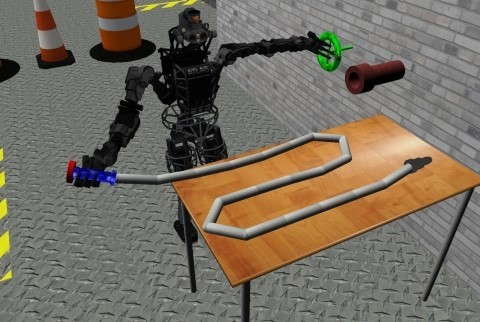
\includegraphics[width=0.7\columnwidth]{pictures/chapter10/darpa_hose_atlas.jpg}
\caption{Bostom Dynamics사의 Atlas 로봇}
\end{figure}

다른 시뮬레이터와 어떤 점이 다른지에 대해 알아보기 위해 가제보 관련 위키를 찾아본 결과, 아래와 같은 특징을 가지고 있었다.

\setcounter{num}{0}

\vspace{\baselineskip}
\noindent\stepcounter{num}
\thenum) 동역학 시뮬레이션: 처음에는 ODE\footnote{\url{http://www.ode.org/}}만 지원했었지만 3.0 버전에 들어오면서 다양한 유저들의 요구에 충족하기 위하여 Bullet\footnote{\url{http://bulletphysics.org/}}, Simbody\footnote{\url{https://simtk.org/home/simbody/}}, DART\footnote{\url{http://dartsim.github.io/}} 등 다양한 물리 엔진을 사용하고 있다.

\vspace{\baselineskip}
\noindent\stepcounter{num}
\thenum) 3차원 그래픽: 가제보에서는 OGRE\footnote{\url{http://www.ogre3d.org/}} (open-source graphics rendering engines)를 이용하여 빛, 그림자, 감촉등을 실감나게 표현하고 있다.

\vspace{\baselineskip}
\noindent\stepcounter{num}
\thenum) 센서와 노이즈 지원: 레이저 레인지 파인더(LRF), 2/3D 카메라, Kinect, 접촉 센서, 힘-토크 센서 등을 가상으로 지원하며 센싱된 데이터에 실제 환경과 비슷하게 노이즈를 포함시킬 수 도 있다.

\vspace{\baselineskip}
\noindent\stepcounter{num}
\thenum) 플러그인 추가 가능: 사용자는 로봇, 센서, 환경 제어 등을 스스로 플러그인 형태로 제작할 수 있도록 API\footnote{\url{http://gazebosim.org/api.html}}를 지원한다.

\vspace{\baselineskip}
\noindent\stepcounter{num}
\thenum) 로봇 모델: PR2, Pioneer2 DX, iRobot Create, TurtleBot 등이 이미 가제보의 모델 파일인 SDF형태로 지원되고 있으며 사용자는 자신의 로봇을 SDF\footnote{\url{http://gazebosim.org/sdf.html}} 형태로 추가할 수도 있다.

\vspace{\baselineskip}
\noindent\stepcounter{num}
\thenum) TCP/IP 데이터 전송: 시뮬레이션은 원격 서버에서도 동작 가능하며 이는 소켓 베이스의 메시지 패싱인 구글 프로토버퍼(Protobufs\footnote{\url{https://code.google.com/p/protobuf/}})를 사용하여 실현하고 있다.

\vspace{\baselineskip}
\noindent\stepcounter{num}
\thenum) 클라우드 시뮬레이션: Gazebo를 Amazon, Softlayer, OpenStack 등에서 사용하기 위하여 CloudSim\footnote{\url{http://cloudsim.io/}}를 사용하여 클라우드 시뮬레이션을 실현하고 있다.

\vspace{\baselineskip}
\noindent\stepcounter{num}
\thenum) 커맨드 라인 툴: 다양한 커맨드 라인 툴을 이용하여 시뮬레이션의 상태 파악 및 제어를 할 수 있다.

\noindent
자~ 그럼 다음 단계에서는 가제보를 설치해보도록 하자.

%-------------------------------------------------------------------------------
\subsection{가제보 설치}

강좌를 작성하는 이 시점에서 가제보의 버전은 4.0 이다. 불과 1년전만 해도 1.9 버전 이였는데 어느새 4.0 버전까지 나왔다. 현재 버전인 4.0 버전을 테스트해본 결과 이를 설치해도 ROS Indigo 에서 따로 패키지로 지원하고 있었서 사용함에 문제가 없었다. 그러나, 일반적으로 ROS 커뮤니티에서는 2.2 버전을 추천하고 있다. 우리는 추천 사항에 따라 2.2 버전을 설치할 것이다. 나중에 4.0을 많이 사용하게 되면 그때가서 강좌를 업데이트 하도록 하겠다. 그럼 우선, 아래와 같이 로봇 모델 양식인 sdformat과 gazebo2 를 설치하자. (gazebo2를 설치하면 2.2버전이 인스톨 된다.)

\vspace{\baselineskip}
\begin{lstlisting}[language=ROS]
$ sudo sh -c 'echo "deb http://packages.osrfoundation.org/gazebo/ubuntu trusty main" > /etc/apt/sources.list.d/gazebo-latest.list'
$ wget http://packages.osrfoundation.org/gazebo.key -O - | sudo apt-key add -
$ sudo apt-get update
$ sudo apt-get install libsdformat1 libsdformat-dev gazebo2 
\end{lstlisting}

가제보를 테스트 하기 위해 아래와 같이 실행해보자. 문제가 없다면 아래의 첨부 그림처럼 가제보가 실행됨을 확인 할 수 있을 것이다. 현재까지는 ROS 와는 상관이 없는 별도의 시뮬레이터라고 볼 수 있다.

\vspace{\baselineskip}
\begin{lstlisting}[language=ROS]
$ gazebo
\end{lstlisting}

\begin{figure}[h]
\centering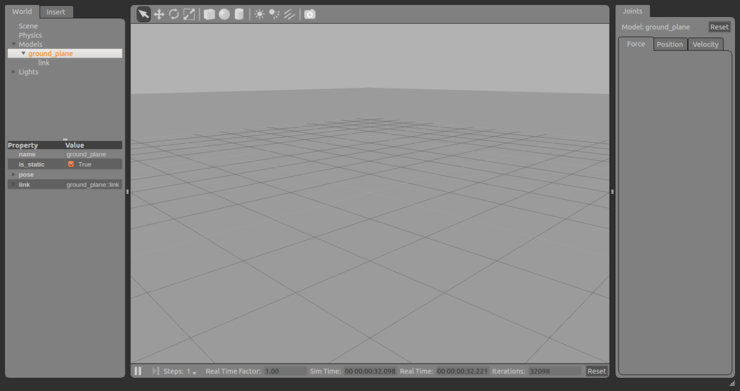
\includegraphics[width=0.9\columnwidth]{pictures/chapter10/gazebo3d.png}
\caption{gazebo 초기 화면}
\end{figure}

이제는 거북이를 가제보 시뮬레이터상에서 동작하기 위하여 관련된 패키지들을 설치해주자. 설치할 패키지로는 가제보와 ROS와의 연동을 위한 gazebo\_ros\_pkgs 메타 패키지와 거북이의 3차원 시뮬레이션 관련 패키지인 kobuki\_desktop 메타 패키지이다.

\vspace{\baselineskip}
\begin{lstlisting}[language=ROS]
$ sudo apt-get install ros-indigo-gazebo-ros ros-indigo-gazebo-plugins ros-indigo-kobuki-desktop
\end{lstlisting}

%-------------------------------------------------------------------------------
\subsection{거북이 시뮬레이션}

아래의 런치파일을 실행하자. 그러면 gazebo, gazebo\_gui, mobile\_base\_nodelet\_manager, robot\_state\_publisher, spawn\_mobile\_base 노드들이 함께 실행되며 아래의 그림과 같이 거북이 가제보 화면에 나타남을 확인 할 수 있다.

\vspace{\baselineskip}
\begin{lstlisting}[language=ROS]
$ roslaunch kobuki_gazebo kobuki_empty_world.launch
\end{lstlisting}

\begin{figure}[h]
\centering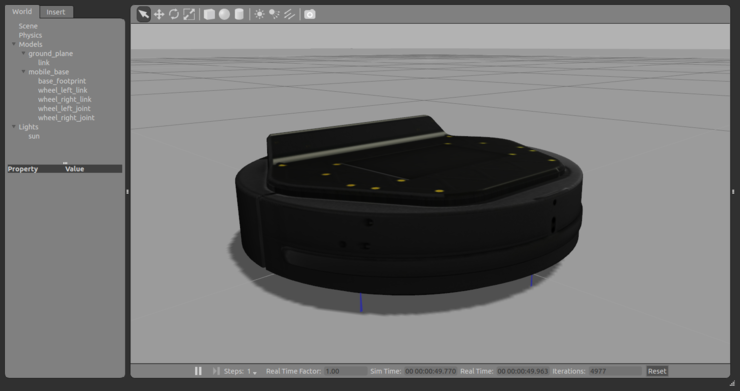
\includegraphics[width=0.9\columnwidth]{pictures/chapter10/gazebo_kobuki.png}
\caption{gazebo상의 kobuki의 3차원 모습}
\end{figure}

위의 상태에서 아래의 원격 제어 런치 파일을 실행하면 가제보 환경 속 가상의 거북이를 제어 가능하다.

\vspace{\baselineskip}
\begin{lstlisting}[language=ROS]
$ roslaunch kobuki_keyop keyop.launch
\end{lstlisting}

그 다음으로,  환경 모델로 기본 설정인 ground\_plane 및 거북이 모델인 mobile\_base 이외에 추가로 테이블 6개, 콘크리트 불럭 3개를 환경 모델로 추가하여 보도록 하자. 관련된 가제보의 world 파일은 아래의 위치에서 에서 찾아 볼 수 있다.  이를 참고하여 자신만의 환경 모델도 만들어 보도록 하자. 굳이 world 파일 직접 수정하지 않아도 가제보에서 직접 모델을 추가해도 된다. 더 자세한 설명은 나중에 가제보에 대한 별도의 특별 강좌를 만들어 보도록 하겠다.\\
world 파일 위치: /opt/ros/indigo/share/kobuki\_gazebo/worlds/playground.world

\vspace{\baselineskip}
\begin{lstlisting}[language=ROS]
$ roslaunch kobuki_gazebo kobuki_playground.launch
\end{lstlisting}

\begin{figure}[h]
\centering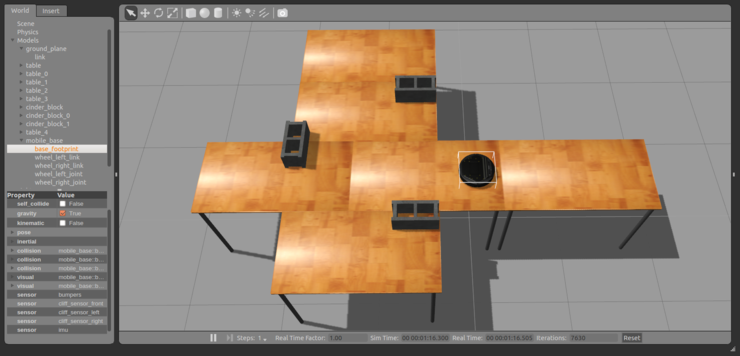
\includegraphics[width=0.9\columnwidth]{pictures/chapter10/gazebo_kobuki_playground.png}
\caption{kobuki\_playground.launch를 시행하였을 때의 모습}
\end{figure}

가제보 환경 속의 가상 거북이 로봇은 외형만을 갖춘게 아니라 위 캡쳐의 좌측 하단의 특성 창에서 확인할 수 있는 것 처럼 각각의 몸체는 충돌을 체크할 수 있고, 위치를 계측하고, 범퍼 3개, 절벽 감지 센서, IMU 센서가 가상으로 사용 가능할 수 있도록 설정되어 있다. 이를 이용한 예제가 아래의 런치 파일이다. 이를 실행하게 되면 가상의 거북이는 테이블 위에서 랜덤하게 이동하면서 절벽을 감지하거나 벽에 부딛쳤을 경우, 그 상황을 회피하여 테이블 위에서 돌아다니게 되어 있다. 학습에 매우 좋은 예제이니 꼭 참고해 보기 바란다.

\vspace{\baselineskip}
\begin{lstlisting}[language=ROS]
$ roslaunch kobuki_gazebo safe_random_walker_app.launch
\end{lstlisting}

거북이 패키지 중 시뮬레이션이 가능한 2가지가 방법을 소개하였다. 하나는 ROS의 3차원 시각화 툴인 RViz 를 이용하는 것이고, 또 다른 하나는 3차원 로봇 시뮬레이터 Gazebo를 이용하는 것이다. 

이 두 강좌는 간단히 시뮬레이션을 소개하는 수준이다. 현재 기획/진행 중인 SLAM과 내비게이션 강좌가 마무리가 되면 가상 공간에서의 시뮬레이션에 대해 좀 더 실직적인 강좌를 작성할 생각이다. 

자~ 다음 강좌는 내비게이션을 위해 필요한 거북이의 제어 개념과 SLAM 등으로 접근해 보도록 하겠다.

%-------------------------------------------------------------------------------